%%% The main file. It contains definitions of basic parameters and includes all other parts.

%% Settings for single-side (simplex) printing
% Margins: left 40mm, right 25mm, top and bottom 25mm
% (but beware, LaTeX adds 1in implicitly)
\documentclass[12pt,a4paper]{report}
\setlength\textwidth{145mm}
\setlength\textheight{247mm}
\setlength\oddsidemargin{15mm}
\setlength\evensidemargin{15mm}
\setlength\topmargin{0mm}
\setlength\headsep{0mm}
\setlength\headheight{0mm}
% \openright makes the following text appear on a right-hand page
\let\openright=\clearpage

%% Settings for two-sided (duplex) printing
% \documentclass[12pt,a4paper,twoside,openright]{report}
% \setlength\textwidth{145mm}
% \setlength\textheight{247mm}
% \setlength\oddsidemargin{14.2mm}
% \setlength\evensidemargin{0mm}
% \setlength\topmargin{0mm}
% \setlength\headsep{0mm}
% \setlength\headheight{0mm}
% \let\openright=\cleardoublepage

%% Generate PDF/A-2u
% \usepackage[a-2u]{pdfx}
%% Character encoding: usually latin2, cp1250 or utf8:
\usepackage[utf8]{inputenc}

\usepackage[unicode]{hyperref}

%% Prefer Latin Modern fonts
\usepackage{lmodern}

%% Further useful packages (included in most LaTeX distributions)
\usepackage{amsmath}        % extensions for typesetting of math
\usepackage{amsfonts}       % math fonts
\usepackage{amsthm}         % theorems, definitions, etc.
\usepackage{amssymb}
\usepackage{bbding}         % various symbols (squares, asterisks, scissors, ...)
\usepackage{bm}             % boldface symbols (\bm)
\usepackage{graphicx}       % embedding of pictures
\usepackage{fancyvrb}       % improved verbatim environment
% \usepackage{natbib}         % citation style AUTHOR (YEAR), or AUTHOR [NUMBER]
\usepackage[nottoc]{tocbibind} % makes sure that bibliography and the lists
			    % of figures/tables are included in the table
			    % of contents
\usepackage{dcolumn}        % improved alignment of table columns
\usepackage{booktabs}       % improved horizontal lines in tables
\usepackage{paralist}       % improved enumerate and itemize
\usepackage[usenames]{xcolor}  % typesetting in color
\usepackage{xspace}

\usepackage[noend]{algpseudocode}
\usepackage{algorithm}
%\usepackage{thmtools, thm-restate}
\algnewcommand{\IIf}[1]{\State\algorithmicif\ #1 \algorithmicthen}
\algnewcommand{\EndIIf}{\unskip\ \algorithmicend\ \algorithmicif}

%%% Basic information on the thesis

% Thesis title in English (exactly as in the formal assignment)
\def\ThesisTitle{Online Bin Stretching:\\ \mbox{Algorithms and Computer Lower Bounds}}

% Author of the thesis
\def\ThesisAuthor{Martin Böhm}

% Year when the thesis is submitted
\def\YearSubmitted{2018}

% Name of the department or institute, where the work was officially assigned
% (according to the Organizational Structure of MFF UK in English,
% or a full name of a department outside MFF)
\def\Department{Computer Science Institute}

% Is it a department (katedra), or an institute (ústav)?
\def\DeptType{Institute}

% Thesis supervisor: name, surname and titles
\def\Supervisor{prof. RNDr. Jiří Sgall, DrSc.}

% Supervisor's department (again according to Organizational structure of MFF)
\def\SupervisorsDepartment{Computer Science Institute}

% Study programme and specialization
\def\StudyProgramme{Computer Science}
\def\StudyBranch{Discrete Models and Algorithms}

% An optional dedication: you can thank whomever you wish (your supervisor,
% consultant, a person who lent the software, etc.)
\def\Dedication{%

\todo{Paste the dedication here in the final version.}
}

\def\DedicationFakke{%

The first person to thank must immediately and irrevocably be my PhD
advisor, Jiří Sgall. Academia has many equally gifted computer
scientists, but he has repeatedly shown to me that one can have both
great talent and great compassion and humanity. He has taught me much
as well as helped me

A special thanks goes to my colleague and frequent coauthor, Pavel
Veselý. We have a student paper together that I am very fond of. He
has submitted a PhD thesis at the same time as me on online packet
scheduling; I recommend the reader to take a look on it as well.

I thank my parents, Michal and Lenka, as well as my sister Kristýna --
you have helped me tremendously whenever I was struggling.

I am grateful to all my friends: Petr Onderka, Lukáš Lánský, Lukáš
Mach, David Marek, Jiří Maršík, Josef Kakrda and many more. Special
thanks to Petr and Tereza for proofreading.

Finally, I would like to thank my partner Tereza Hulcová for
everything.

}

% Abstract (recommended length around 80-200 words; this is not a copy of your thesis assignment!)
\def\Abstract{%
Abstract.
}

% 3 to 5 keywords (recommended), each enclosed in curly braces
\def\Keywords{%
{bin stretching} {online scheduling} {bin packing} {online algorithms} {computer search} }

%% The hyperref package for clickable links in PDF and also for storing
%% metadata to PDF (including the table of contents).
%% Most settings are pre-set by the pdfx package.
\hypersetup{unicode}
\hypersetup{breaklinks=true}

% Definitions of macros (see description inside)
%%% This file contains definitions of various useful macros and environments %%%
%%% Please add more macros here instead of cluttering other files with them. %%%

%%% Minor tweaks of style

% These macros employ a little dirty trick to convince LaTeX to typeset
% chapter headings sanely, without lots of empty space above them.
% Feel free to ignore.
\makeatletter
\def\@makechapterhead#1{
  {\parindent \z@ \raggedright \normalfont
   \Huge\bfseries \thechapter. #1
   \par\nobreak
   \vskip 20\p@
}}
\def\@makeschapterhead#1{
  {\parindent \z@ \raggedright \normalfont
   \Huge\bfseries #1
   \par\nobreak
   \vskip 20\p@
}}
\makeatother

% This macro defines a chapter, which is not numbered, but is included
% in the table of contents.
\def\chapwithtoc#1{
\chapter*{#1}
\addcontentsline{toc}{chapter}{#1}
}

% Draw black "slugs" whenever a line overflows, so that we can spot it easily.
\overfullrule=1mm

%%% Macros for definitions, theorems, claims, examples, ... (requires amsthm package)

\theoremstyle{plain}
\newtheorem{thm}{Theorem}
\newtheorem{lem}[thm]{Lemma}
\newtheorem{clm}[thm]{Claim}
\newtheorem{obs}[thm]{Observation}
\newtheorem{goodsit}{Good Situation}
\newtheorem{gengoodsit}{Good Situation} % to avoid pdftex warning about duplicate labels

\theoremstyle{definition}
\newtheorem{dfn}{Definition}
\newtheorem{prb}{Problem}

\theoremstyle{remark}
\newtheorem*{cor}{Corollary}
\newtheorem*{rem}{Remark}
\newtheorem*{example}{Example}

%%% An environment for proofs

%%% FIXME %%% \newenvironment{proof}{
%%% FIXME %%%   \par\medskip\noindent
%%% FIXME %%%   \textit{Proof}.
%%% FIXME %%% }{
%%% FIXME %%% \newline
%%% FIXME %%% \rightline{$\square$}  % or \SquareCastShadowBottomRight from bbding package
%%% FIXME %%% }

%%% An environment for typesetting of program code and input/output
%%% of programs. (Requires the fancyvrb package -- fancy verbatim.)

\DefineVerbatimEnvironment{code}{Verbatim}{fontsize=\small, frame=single}

%%% The field of all real and natural numbers
\newcommand{\R}{\mathbb{R}}
\newcommand{\N}{\mathbb{N}}

%%% Useful operators for statistics and probability
\DeclareMathOperator{\pr}{\textsf{P}}
\DeclareMathOperator{\E}{\textsf{E}\,}
\DeclareMathOperator{\var}{\textrm{var}}
\DeclareMathOperator{\sd}{\textrm{sd}}

%%% Transposition of a vector/matrix
\newcommand{\T}[1]{#1^\top}

%%% Various math goodies
\newcommand{\goto}{\rightarrow}
\newcommand{\gotop}{\stackrel{P}{\longrightarrow}}
\newcommand{\maon}[1]{o(n^{#1})}
\newcommand{\abs}[1]{\left|{#1}\right|}
\newcommand{\dint}{\int_0^\tau\!\!\int_0^\tau}
\newcommand{\isqr}[1]{\frac{1}{\sqrt{#1}}}

%%% Various table goodies
\newcommand{\pulrad}[1]{\raisebox{1.5ex}[0pt]{#1}}
\newcommand{\mc}[1]{\multicolumn{1}{c}{#1}}


% custom macros

\newcommand\binstretch{{\sc Online Bin Stretching}\xspace}
\newcommand\binpacking{{\sc Bin Packing}\xspace}
\newcommand\scheduling{\textsc{Online Scheduling}\xspace}
\newcommand\Nat{\mathbb{N}}

\newcommand\eps\varepsilon
\newcommand\calA{{\mathcal A}}
\newcommand\Cprime{{\mathcal C'}}
\newcommand\calB{{\mathcal B}}
\newcommand\calC{{\mathcal C}}
\newcommand\calD{{\mathcal D}}
\newcommand\calE{{\mathcal E}}
\newcommand\calF{{\mathcal F}}
\newcommand\calH{{\mathcal H}}
\newcommand\calI{{\mathcal I}}
\newcommand\calL{{\mathcal L}}
\newcommand\calR{{\mathcal R}}
\newcommand\Aprime{{\mathcal A'}}
\newcommand{\hmodfour}{{h}}
\newcommand{\before}{\leftarrow}

\newcommand{\Rbar}{R_{\mbox{\rm\scriptsize first}}}
\newcommand\mycase[1]{\vspace{0.4ex}\noindent{\bf #1}}
\newcommand\mycasesp[1]{\vspace{1ex}\noindent{\bf #1}}

\def\indentskip{\hskip 1.5em}
\def\indentskiptwodigit{\hskip 1em}

\newcommand\algobox[1]{\begin{center}
\fbox{\parbox[c]{0.95\textwidth}{#1}}
\end{center}
}

\def\O{{\mathcal{O}}}
\let\csc=\textsc
\def\GSFF#1{{\rm\csc{GSFF(#1)}}}
\def\FF{{\rm\csc{First Fit}}\xspace}
\def\tbalg{\textsc{Evasive}\xspace}
\def\SP{{\textsc{Large Item Early}}\xspace}
\def\enumparams{\itemsep1pt \parskip0pt}

\def\step#1{{\ref{fp:#1}}}
\def\eq#1{{(\ref{eq:#1})}}
\def\gs#1{GS\ref{lem:gs#1}}

% box related macros
\def\frombox#1{\hbox to 1em{{\bf #1}\hss}}
\def\tobox#1{\hbox to 2.3em{{\bf #1}\hss}}
\def\arrow{\hbox to 1.5em{$\rightarrow$}}

\makeatletter
\newcommand*{\defeq}{\mathrel{\rlap{%
                     \raisebox{0.3ex}{$\m@th\cdot$}}%
                     \raisebox{-0.3ex}{$\m@th\cdot$}}%
                     =}
\makeatother


\newcommand\ALG{\mathrm{ALG}}
\newcommand\OPT{\mathrm{OPT}}
% macros for the lower bound chapter
\renewcommand\Game{{\mathrm{BSG}}}
\newcommand\algo{\textsc{Algorithm}\xspace}
\newcommand\adversary{\textsc{Adversary}\xspace}
\newcommand\evaladv{\textsc{EvaluateAdversary}\xspace}
\newcommand\evalalg{\textsc{EvaluateAlgorithm}\xspace}
\newcommand\minimax{\textsc{Minimax}\xspace}
\newcommand\Main{\textsc{Main}\xspace}
\newcommand\Sequential{\textsc{Sequential}\xspace}

\newcommand\Test{\textsc{Test}\xspace}
\newcommand\DynprogMax{\textsc{DynprogMax}\xspace}
\newcommand\Query{\textsc{Query}\xspace}
\newcommand\MaxFeas{\textsc{MaxFeas}\xspace}
\newcommand\bfd{\textsc{Best Fit Decreasing}\xspace}
\newcommand\obf{\textsc{Online Best Fit}\xspace}
\newlength{\elseskiplen}
\settowidth{\elseskiplen}{Else: }
\newcommand\elseskip{\hskip\elseskip}


\newcommand\todo[1]{\textcolor{red}{#1}}

% Title page and various mandatory informational pages
\begin{document}
%%% Title page of the thesis and other mandatory pages

%%% Title page of the thesis

\pagestyle{empty}
\hypersetup{pageanchor=false}
\begin{center}

\centerline{\mbox{
\includegraphics[width=166mm]{img/logo-en.pdf}}}

\vspace{-8mm}
\vfill

{\bf\Large DOCTORAL THESIS}

\vfill

{\LARGE\ThesisAuthor}

\vspace{15mm}

{\LARGE\bfseries\ThesisLargeTitle}

\vfill

\Department

\vfill

\begin{tabular}{rl}

Supervisor of the doctoral thesis: & \Supervisor \\
\noalign{\vspace{2mm}}
Study programme: & \StudyProgramme \\
\noalign{\vspace{2mm}}
Study branch: & \StudyBranch \\
\end{tabular}

\vfill

% Zde doplňte rok
Prague \YearSubmitted

\end{center}

\newpage

%%% Here should be a bound sheet included -- a signed copy of the "doctoral
%%% thesis assignment". This assignment is NOT a part of the electronic
%%% version of the thesis. DO NOT SCAN.

%%% A page with a solemn declaration to the doctoral thesis

\openright
\hypersetup{pageanchor=true}
\pagestyle{plain}
\pagenumbering{roman}
\vglue 0pt plus 1fill

\noindent
I declare that I carried out this doctoral thesis independently, and only with the cited
sources, literature and other professional sources.

\medskip\noindent
I understand that my work relates to the rights and obligations under the Act No.~121/2000 Sb.,
the Copyright Act, as amended, in particular the fact that the Charles
University has the right to conclude a license agreement on the use of this
work as a school work pursuant to Section 60 subsection 1 of the Copyright Act.

\vspace{10mm}

\hbox{\hbox to 0.5\hsize{%
In ........ date ............	% FIXME!
\hss}\hbox to 0.5\hsize{%
signature of the author
\hss}}

\vspace{20mm}
\newpage

%%% Dedication

\openright

\noindent
\Dedication

\newpage

%%% Mandatory information page of the thesis

\openright

\vbox to 0.5\vsize{
\setlength\parindent{0mm}
\setlength\parskip{5mm}

Title:
\ThesisTitle

Author:
\ThesisAuthor

\DeptType:
\Department

Supervisor:
\Supervisor, \SupervisorsDepartment

Abstract:
\Abstract

Keywords:
\Keywords

\vss}

\newpage

\openright
\pagestyle{plain}
\pagenumbering{arabic}
\setcounter{page}{1}


%%% A page with automatically generated table of contents of the doctoral thesis

\tableofcontents

%%% Each chapter is kept in a separate file
\chapter{Introduction}\label{chap:intro}

\section{An example}\label{sec:example}

We start with an example to illustrate the problem central to this thesis.

A number $m$ of containers arrive at a shipping center. It is noted
that all containers are at most $66$ percent full. The items in the
containers are too numerous to be individually labeled, yet all items
must be unpacked and scanned for illicit and dangerous material. After
the scanning, the items arrive at a conveyor belt one by one and they must
be speedily repackaged into the original containers for further shipping.

Our question is: Does there exist a fast computer program which can
repackage the items into the original containers without any
reassignments?

We will settle our central question later in the thesis in the
affirmative (the program exists). Before proceeding with the formal
definitions, let us consider where the difficulty of this problem
lies.

First, let us imagine that we are in the same shipping center, but in
this case we receive two $99$ percent loaded containers. Suppose that
the first item arriving through the scanner is of size $50\%$. We can
choose either container for it, and it is clearly not a wrong choice,
as they are identical.

After storing the first item, a second item arrives through the
scanner, this one of size $47\%$ of the size of the container. We have
a choice to make: Do we pack it with the first item or not? See
Figure~\ref{fig:ninetynine} for illustration.

\begin{figure}[th]
\begin{center}
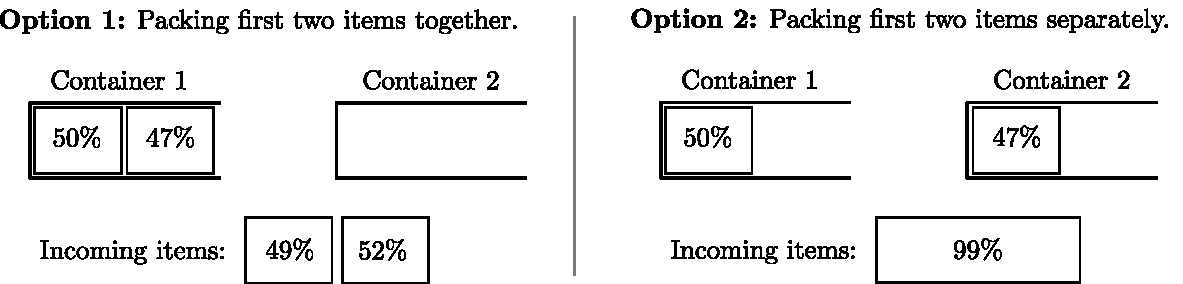
\includegraphics[width=\textwidth]{img/ninetynine.pdf}
\end{center}
\caption{Two possible choices for repacking containers that are $99\%$ full.}
\label{fig:ninetynine}
\end{figure}


A quick thought gives us that there is no good choice here: If we pack
it with the first item, we get a container that is 97 percent loaded,
but then, to our dismay, we receive two items of sizes $49\%$ and
$52\%$, respectively -- and those cannot be packed together. On the
other hand, if we pack the first two items separately into two
containers, we can find that the third item is a large crate taking up
$99\%$ of the container's size, and we have no more containers to
choose from!

\paragraph{A lower bound.} In the last few paragraphs, we have seen
that repacking two containers that are $99\%$ full is impossible
without additional information on their contents. Can we actually get
a lower number than $99\%$ using only simple ideas? The answer is yes;
we can show that we cannot repack two containers that are strictly
more than $75\%$ full. The thought process is explained in Figure~\ref{fig:example-lowerbound}.

The key decision of any algorithm (for containers loaded below $75\%$,
where a repacking algorithm might exist) is then whether to pack
sizable items together and increase the total loaded volume of one
container, or pack them separately to avoid a potentially unsolvable
situation.

\begin{figure}[th]
\begin{center}
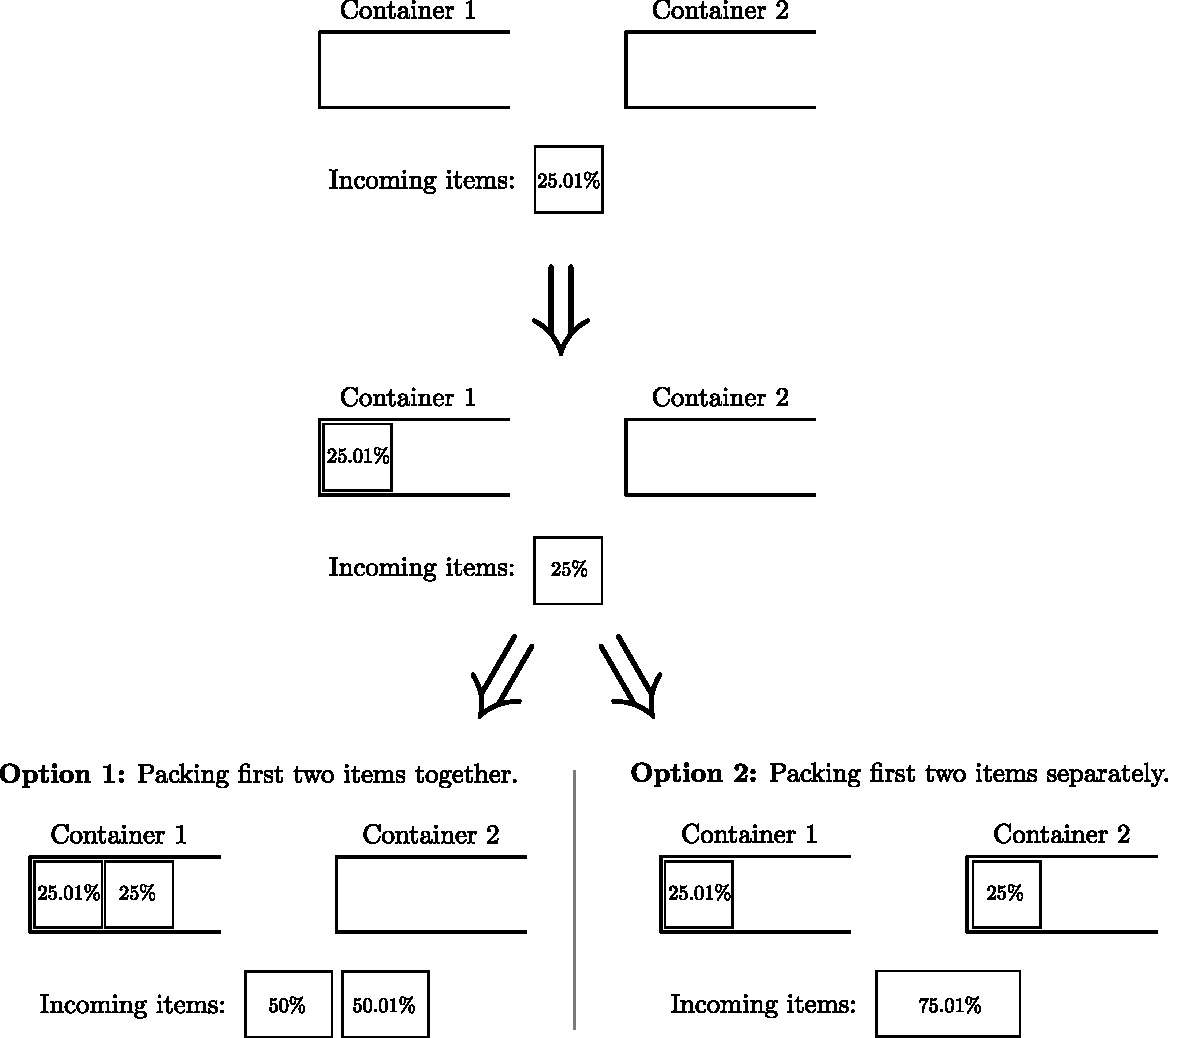
\includegraphics[width=\textwidth]{img/example-lowerbound.pdf}
\end{center}
\caption[A visual proof that two containers with original load of $75.01\%$ cannot
be repackaged without any reassignments.]{A visual proof that two containers with original load of $75.01\%$ cannot
be repackaged without any reassignments. A careful reader will observe that the number
of containers is not important here; a similar visual proof can be created for any
number of containers.}
\label{fig:example-lowerbound}
\end{figure}


% The most famous algorithmic problem dealing with online assignment is
% arguably {\sc Online Bin Packing}.  In this problem, known since the
% 1970s, items of size between $0$ and $1$ arrive in a
% sequence and the goal is to pack these items into the least number of
% unit-sized bins, packing each item as soon as it arrives.

% \binstretch, which has been introduced by Azar and Regev in
% 1998~\cite{azar98,azar01}, deals with a similar online
% scenario. Again, items of size between $0$ and $1$ arrive in a
% sequence, and the algorithm needs to pack each item as soon as it
% arrives, but there are the following differences: (i) The packing
% algorithm knows $m$, the number of bins that an optimal offline
% algorithm would use, and must also use only at most $m$ bins, and (ii)
% the packing algorithm can use bins of capacity $R$ for some $R\geq
% 1$. The goal is to minimize the stretching factor $R$.

% In general, the term ``semi-online'' refers to algorithms that,
% compared to online algorithms, have some additional global information
% about the instance of the problem or have another advantage. We have
% formulated \binstretch as a semi-online bin packing variant, where the
% algorithm has the additional information that the optimal number of
% bins is $m$ and at the same time the algorithm has the advantage of
% using bins of larger capacity.

% Taking another view, \binstretch can also be thought of as a
% semi-online scheduling problem, in which we schedule jobs arriving one
% by one in an online manner on exactly $m$ machines, with the objective
% to minimize the makespan, i.e., the length of the resulting
% schedule. Here the additional information is that the optimal offline
% algorithm could schedule all jobs with makespan $1$. Our task is to
% present an algorithm with makespan being at most $R$.

%\smallskip\noindent
%{\bf Motivation.} We give two applications of \binstretch.
%
%{\it Server upgrade.} This application has first appeared
%in~\cite{azar98}. In this setting, an older server (or a server
%cluster) is streaming a large number of files to the newer server
%without any guarantee on file order. The files cannot be split between
%drives. Both servers have $m$ disk
%drives, but the newer server has a larger capacity of each drive. The
%goal is to present an algorithm that stores all incoming files from
%the old server as they arrive.
%


% \todo{Below intro for threebins.}

% \section{Introduction}

% The most famous algorithmic problem dealing with online assignment is
% arguably {\sc Online Bin Packing}. In this problem, known since the
% 1970s, items of size between $0$ and $1$ arrive in a
% sequence and the goal is to pack these items into the least number of
% unit-sized bins, packing each item as soon as it arrives.

% \binstretch, which was introduced by Azar and Regev in 1998~\cite{azar98,azar01}, deals with a
% similar online scenario. Again, items of size between $0$ and $1$
% arrive in a sequence, and the algorithm needs to pack them as soon as
% each item arrives, but it has two advantages: (i) The packing
% algorithm knows $m$, the number of bins that an optimal offline
% algorithm would use, and must also use only at most $m$ bins, and (ii)
% the packing algorithm can use bins of capacity $R$ for some
% $R\geq 1$. The goal is to minimize the stretching factor $R$.

% While formulated as a bin packing variant, \binstretch can also be
% thought of as a semi-online sche\-du\-ling problem, in which we schedule
% jobs in an online manner on exactly $m$ machines, before any execution
% starts.  We have a guarantee that the optimum offline algorithm could
% schedule all jobs with makespan $1$. Our task is to present an online
% algorithm with makespan of the schedule being at most $R$.

% % \iffalse % motivation can be skipped to save space
% \subsection{Motivation} We give two applications of \binstretch.

% {\it Server upgrade.} This application has originally appeared
% in~\cite{azar98}. In this setting, an older server (or a server
% cluster) is streaming a large number of files to the newer server
% without any guarantee on file order. The files cannot be split between
% drives. Both servers have $m$ disk
% drives, but the newer server has a larger capacity of each drive. The
% goal is to present an algorithm that stores all incoming files from
% the old server as they arrive.

% {\it Shipment checking.} A number $m$ of containers arrive at a
% shipping center. It is noted that all containers are at most $p \le 100$ percent
% full. The items in the containers are too numerous to be individually
% labeled, yet all items must be unpacked and scanned for illicit and dangerous
% material. After the scanning, the items must be speedily
% repackaged into the containers for further shipping.
% In this scenario, an algorithm with stretching factor $100/p$
% can be used to repack the objects into containers in an online manner.
% % \fi

% \subsection{History}  
% \binstretch was first proposed by Azar and Regev in~\cite{azar98,azar01}.
% Already before this, a matching upper and lower bound of $4/3$ for two bins
% had appeared~\cite{KeKoST97}.
% %The original lower bound of $4/3$ for three bins has appeared even
% %before that, in~\cite{KeKoST97}, for two bins together with a matching
% %algorithm.  
% Azar and Regev extended this lower bound to any number
% of bins and gave an online algorithm with a stretching factor $1.625$.

% The problem has been revisited recently, with both lower bound
% improvements and new efficient algorithms. On the algorithmic side,
% Kellerer and Kotov~\cite{kellerer2013} have achieved a stretching
% factor $11/7 \approx 1.57$ and Gabay et al.~\cite{gabay2013} 
% have achieved $26/17 \approx
% 1.53$. The best known general algorithm with stretching factor $1.5$
% was presented by the authors of this paper in \cite{bsvsv16}.

% In the case with only three bins, the previously best
% algorithm was due to Azar and Regev~\cite{azar98}, with a stretching
% factor of $1.4$.

% On the lower bound side, the lower bound $4/3$ of~\cite{azar98} was
% surpassed only for the case of three bins by Gabay et
% al.~\cite{gabay2013lbv2}, who show a lower bound of $19/14\approx
% 1.357$, using an extensive computer search. The preprint
% \cite{gabay2013lbv2} was updated in 2015 \cite{gabay2013lbv3} to
% include a lower bound of $19/14$ for four bins.

% A preliminary version of this work appeared in WAOA 2014
% \cite{bsvsv14} and SOFSEM 2016~\cite{bohm16}.

% % \smallskip\noindent
% \subsection{Related work.} The NP-hard problem \binpacking was originally
% proposed by Ullman~\cite{ullman71} and Johnson~\cite{johnson73} in the
% 1970s. Since then it has seen major interest and progress, see the
% survey of Coffman et al.~\cite{coffman13} for many results on
% classical Bin Packing and its variants. While our problem can be seen
% as a variant of {\sc Bin Packing}, note that the algorithms cannot
% open more bins than the optimum and thus general results for
% \binpacking do not translate to our setting.

% As noted, \binstretch can be formulated as the online scheduling on $m$ identical
% machines with known optimal makespan. Such algorithms were studied and
% are important in designing constant-competitive algorithms without the
% additional knowledge, e.g., for scheduling in the more general model
% of uniformly related machines~\cite{AsAFPW97,BeChKa00,EbJaSg09}.

% For scheduling, also other types of semi-online algorithms are
% studied. Historically first is the study of ordered sequences with
% non-decreasing processing times~\cite{Graham69}. Most closely
% related is the variant with known sum of all processing times studied
% in~\cite{KeKoST97} and the currently best results are a lower bound of
% $1.585$ and an algorithm with ratio $1.6$, both
% from~\cite{DBLP:journals/tcs/AlbersH12}. Note that this shows,
% somewhat surprisingly, that knowing the actual optimum gives a
% significantly bigger advantage to the online algorithm over knowing
% just the sum of the processing times (which, divided by $m$, is a
% lower bound on the optimum).


\section{The online model of computation}

Before we continue with the investigation of the problem of repacking
containers, we specify the model of computation that we are
considering.

For those not in the know of the theoretical computer science
terminology, an \textit{online algorithm} conjures an image of a
program which is hosted on a server on the internet. This may indeed
be so, but the definition actually predates the internet and goes to
the 1970s, where the word ``online'' implied something arriving
literally ``on a line'', such as on a conveyor belt.

In the online model, the input to the algorithm is not known in
advance, but it arrives sequentially, one by one -- exactly like
luggage on the conveyor belt. After each part of the input arrives,
the algorithm must \textit{immediately} and \textit{irrevocably}
decide what to do with this particular piece of the input. Most
commonly, the decision is where to send a packet, which processor core
should be selected for the current task, or which container should be
used to pack the incoming item. As mentioned, after a decision is
made, it cannot be reverted. 

Only after a decision is made, the next item in the sequence is
revealed to the algorithm, and the same decision process is repeated;
of course even if two items arrive which are exactly the same, the
algorithm can decide differently on them, since it knows the history
of the instance.

After the entire input is processed, we look at the whole output of
the algorithm and consider it a \emph{solution} of the online problem.
Naturally, the resulting solution is also a valid solution for the
original non-online optimization problem, but usually is worse than
what a normal polynomial-time algorithm for that optimization problem
would produce.

\begin{dfn}
An \emph{online problem} is an optimization problem where some part of
the input instance arrives sequentially, one by one. After each part
arrives, it must be processed immediately and irrevocably, and the
next part of the input instance arrives only after the processing of
the previous part is complete.

An \emph{online algorithm} is an algorithm that outputs some solution
of an online problem. Given an instance $I$ of the online problem, we
can measure the performance of the online algorithm by its output's
\emph{value} on the function being optimized. We denote its value on
instance $I$ as $\ALG(I)$.
\end{dfn}

As examples of online problems, we can list the two that are arguably
the most well-studied: scheduling and bin packing.

\begin{prb}[\scheduling]~
\smallskip

\noindent\textbf{Input:}
\begin{itemize}
\item A number $m$ -- the number of available equal-speed machines.
\item A sequence $j_1, j_2, …, j_n$ of jobs, arriving online (one by one). Each job $j$ has its own non-negative \emph{processing time} $p(j)$. The processing time is revealed when the job arrives. The number of jobs $n$ is not known in advance.
\item Once a job appears, the algorithm must assign the job to one machine; the next job is revealed after the decision is made.
\end{itemize}

\noindent\textbf{Output:} A schedule (assignment) of jobs to machines,
along with the makespan, which is the sum of the processing times on
the busiest machine.

\noindent\textbf{Goal:} Design an online algorithm that minimizes the
makespan.
\end{prb}

\begin{prb}[\binpacking]~
\smallskip

\noindent\textbf{Input:}
\begin{itemize}
\item A sequence $i_1, i_2, …, i_n$ of items, arriving online (one by one). Each item $i$ has its own non-negative \emph{size} $s(i), s(i) \le 1$. The size is revealed when the item arrives.
\item Once an item appears, it must be assigned to a \emph{bin} such that the total load of the bin after the assignment is at most $1$. The algorithm can open a new bin (with load $0$) at any time, and can open any number of bins.
\end{itemize}

\noindent\textbf{Output:} A number of bins used by the algorithm $B$, as well as
the assignment of all input items into these bins.

\noindent\textbf{Goal:} Design an online algorithm that minimizes the number of bins $B$.
\end{prb}

\medskip

The goal of algorithm designers is not only designing algorithms that
perform well in practice, but also those that \emph{verifiably}
perform well. Since online algorithms are designed only for
optimization problems, one could suggest to compute the value of the
best possible online algorithm for the problem and compare our
algorithm to that value. This is actually quite hard, since in almost
all cases there is no good way to compute the value of the optimal
online algorithm.

Instead, we compare our algorithm's performance to an optimum that
actually is not online at all, but has access to the whole input at
the same time. We define it as follows: 

\begin{dfn}\label{dfn:compratio}
An \emph{offline optimal algorithm} is an algorithm that optimally
solves the online problem when given the entirety of the instance at the start
of the program. On an instance $I$, we denote its value as $\OPT(I)$.

For a minimization problem, we say an online algorithm has
\emph{competitive ratio $c$}, if for all instances $I$,

\[ \ALG(I) \le c \cdot \OPT(I). \]

For a maximization problem, we say an online algorithm has
\emph{competitive ratio $c$} if for all $I$,

\[ \OPT(I) \le c \cdot \ALG(I). \]

\end{dfn}

It might seem confusing to some readers that the competitive ratio is
differently defined for minimization and maximization problems; this
is done so chiefly to make sure that the competitive ratio $c$ is
always in the interval $[1,\infty]$ of real numbers.

So far we have not spoken at all about the running time of online
algorithms. This was intentional: there are no time or space
restrictions on their computation. All we need is that they are
algorithms, i.e., they finish in finite time. Despite this relaxed
view of algorithmic runtime, almost all online algorithms turn out to
run in polynomial time, many even in linear time.

% \todo{Mention that the computational complexity is unlimited. Also check
% the definitions.}

\section{Knowing a little in advance: the semi-online model}

As we discussed above, an online algorithm cannot work with any assumptions
about the input or its order -- which means that if an online algorithm works
excellently on larger input instances but poorly on a sequence of short length,
its performance will be judged exactly on those short sequences.

One can easily see that ``assuming nothing'' is both a great advantage
and at the same time a big disadvantage of the online computation
model. Consider for instance the internet -- while our algorithms
should behave well under any scenario, it is not true that the very
worst scenario will always come true. Indeed, many routing and
scheduling algorithms make use of previously computed statistics and
assumptions about the data to behave well only in an average case or
even just as a \textit{heuristic}, i.e. without any provable guarantees.

If we wish to make our rule of ``assuming nothing'' weaker, we have
several different options, all already studied in literature:

\begin{enumerate}

\item We could assume that the incoming items are not random, but
are coming from a probabilistic distribution whose parameters we know.
This is called \textit{stochastic online optimization}.

\item We could assume that we are given some advice from an entity
that has knows much more about the input than we do (a likely
candidate for such an oracle would be NSA). While this entity can give
us any advice at all, the information must be relatively small, for
the model to make sense. After our algorithm receives this arbitrary
but limited advice, it must make use of it to solve the online problem
in an effective way. This model is called \textit{online optimization
with advice}.

\item There is a common sense weakening of the \textit{optimization
with advice} model from the previous point, and we can describe it
with an example. Suppose that our online algorithm is packing a
sequence of apples into crates as best as it can. If we assume any
advice at all, the algorithm could receive some information about the
average curvature of the current batch of apples. The curvature may
be potentially useful for packing, but clearly in real life there is no
way an apple orchard can provide such an oddly specific piece of data.

A much more reasonable request would be to provide the total number of
apples, the total weight of the apples, or the estimated quality of
the current season's fruit. In other words, in this model, we get a
reasonable and pre-defined piece of information about the instance in
advance, but our algorithms still need to solve the instance in an
online way.

This model is called \textit{semi-online optimization}, and it is the
one we focus on in this thesis. We mention the other two models briefly
in Section~X. \todo{Mention related work section.}

\end{enumerate}
\section{The bin stretching problem}\label{sec:binstretchdef}

Let us return to our semi-online container repacking problem from
Section~\ref{sec:example}, which we now define formally:

\begin{prb}[\binstretch]~

\noindent\textbf{Input:}

\begin{itemize}
\item An integer $m$ --  the number of allowed bins. All bins are initially empty.
\item A sequence of items $I=i_1, i_2, \ldots$ given online one by one. Each item has
a {\it size} $s(i) \in [0,1]$ and must be packed immediately and irrevocably into one of the $m$ bins; the next item
is revealed only after the previous one is packed.
\end{itemize}

\noindent\textbf{Parameter:} The {\it stretching factor} $R\geq 1$.

\noindent\textbf{Output:} Partitioning (packing) of $I$ into bins $B_1,\ldots,B_m$
so that $\sum_{i\in B_j}s(i)\leq R$ for all $j=1,\ldots,m$.

\noindent\textbf{Guarantee:} there exists a packing of all items in $I$ into $m$
bins of capacity $1$. 

\noindent\textbf{Goal:} Design an online algorithm with the stretching factor $R$
as small as possible which packs all input sequences satisfying the
guarantee.
\end{prb}
\medskip

The aforementioned stretching factor is just another name for the
competitive ratio of our algorithm in the standard terminology of
online algorithms (see Definition~\ref{dfn:compratio}). Still, when designing
algorithms for \binstretch it makes more sense to think about it as a
parameter, as a maximum load that we want to ensure in all bins.

As we can see from the nomenclature above -- bins, load, packing -- we
will think of the problem as if it were related to \binpacking
(defined in Section~X). This is also how the literature discusses the
problem.  It is however important to keep in mind that the problem is
not a variant of \binpacking -- the crucial difference is that we are
not allowed to open as many bins as we want, which is allowed in
\binpacking.

In fact, \binstretch is a variant of \scheduling (also defined in
Section~X). In the scheduling terminology, we would call it
\textsc{Online Scheduling with Known Optimal Makespan}, and we would
describe it this way:

 \noindent
\textbf{Input:}

\begin{itemize}
\item An integer $m$ -- a number of identical (equally fast) \emph{machines};
\item A sequence of \emph{jobs} $I=i_1, i_2, \ldots$ given online one by one. Each job has
a \textit{processing time} $s(i) \in [0,1]$ and must be assigned immediately and irrevocably
to one of the machines. The jobs cannot be paused or reassigned later.
\end{itemize}

\noindent
\textbf{Output:} A \emph{schedule} assigning all input items to $m$ machines, with the
load of the busiest machine (called \emph{makespan}) being some value
$R$.

\noindent
\textbf{Guarantee:} There exists a schedule which assigns all jobs so that
the makespan is at most $1$.

\noindent
\textbf{Goal:} Design an online algorithm minimizing the makespan $R$.
\smallskip


\paragraph{A pinch of notation.} For a bin $B$, we define the
\textit{load of the bin} $s(B) = \sum_{i \in B} s(i)$. Unlike
$s(i)$, $s(B)$ can change during the course of the algorithm, as we
pack more and more items into the bin. To easily differentiate between
items, bins and lists of bins, we use lowercase letters for items
($i$, $b$, $x$), uppercase letters for bins and other sets of items
($A$, $B$, $X$), and calligraphic letters for lists of bins ($\calA$,
$\calC$, $\calL$).

\paragraph{Input scaling.} We have defined \binstretch as a problem
where all input items are of size between $0$ and $1$; in other words,
all sizes are set up so that the guaranteed optimum packing is $1$.
This is natural for a generic definition, but writing and especially
adding fractions such as $\frac{1}{2}$ and $\frac{7}{16}$ becomes
tiresome after a while.

Therefore, in all three sections of the thesis, we rescale the
instance so that the capacity of the bins in the optimum packing
becomes some positive integer $S \ge 1$ and the capacity of a bin for
the algorithm will also be some positive integer $R \ge S$. The
resulting stretching factor will therefore be $R/S$.

It is worthwhile to keep in mind that our rescaling still allows
fractional values; while bins have integral capacity both for the
algorithm and for the optimal guarantee, the input item size $s(i)$
can be any value in the interval $(0,S]$.

\section{Bin Stretching as a game}\label{sec:binstretchgame}

A basic and essential feature of any online problem -- with
\binstretch being no exception -- is that any online algorithm is
actually an algorithm for strategy in a two-player game.

What do we mean by that? If we recall the definition of the
competitive ratio, we see that we measure our algorithm on the actual
worst case that can happen, and this worst case is actually
\emph{adapting} to what the algorithm does for the preceeding items.

Therefore, we can see the creator of the worst case as a person who
plays a game with our algorithm, waiting for its move (in our case,
where it packs the previous item) and then sending the next item so
that the algorithm's decision is the worst possible.

In the online algorithm literature, we call this player
\adversary. The other player, naturally, is called \algo.

\begin{dfn} 
A \emph{combinatorial two-player game} is a game with two
players with perfect information (the game state is fully revealed to
both players). Each player has a set of moves (which does not need to
be symmetric) and they alternate in selecting one move each.

A set of game states are denoted as winning the game for the first
player and another set as winning for the second player. The two sets
are known to both players in advance.

A player \emph{wins} the game if it reaches its own winning state in a
finite set of moves. A player has a \emph{winning strategy} if
it can reach a winning state regardless of the moves of the other
player.
\end{dfn}

\todo{Find reference for the earliest mention of this.}

\begin{thm}
Fix a target competitive ratio $c$. An online problem along
with $c$ corresponds to a combinatorial two-player game between
players \algo and \adversary. The player \algo has a winning
strategy if and only if there exists a $c$-competitive algorithm for
the online problem. The player \adversary has a winning strategy
if and only if no $c$-competitive algorithm exists.
\end{thm}

One can argue (in jest) that the main consequence of this theorem is
that the literature on online algorithms loves to use terminology from
combinatorial game theory; it is the author's personal experience that
imagining an adversary and constantly thinking about its moves is
useful when designing a new online algorithm.

However, the more important consequence for us is that if we can
evaluate the entire decision tree for a game that corresponds to an
online problem with a fixed ratio $c$, we can learn whether a
$c$-competitive algorithm exists or not. There is a classical
algorithm for evaluating a game tree called \emph{the minimax
algorithm} which is effective as long as the tree can be somehow
bounded.

So far, everything we stated about game theory applies in full
generality, but we will focus on \binstretch exclusively; therefore,
we restate the game that corresponds to \binstretch:

\begin{dfn}
Fix a number of bins $B$ and a stretching factor $S$. The \emph{bin stretching game}
is defined as follows:

\begin{enumerate}
\item It is a two-player game between \algo and \adversary, and the player \adversary starts.
\item The player \adversary moves by sending any item $i \in (0,1]$ with the restriction
that $i$ along with all previous items can be packed into $B$ bins of capacity $1$.
\item The player \algo moves by selecting a bin where the item is packed.
\end{enumerate}

The winning states are defined thus:
\begin{itemize}
\item A state is winning for \algo if all bins are packed strictly below $S$ and \adversary
has cannot make any further moves.
\item A state is winning for \adversary if one bin has total load at least $S$.
\end{itemize}
\end{dfn}

As you can see, we have formulated the bin stretching game with the
player \algo trying to pack strictly below $S$. This way, a winning
strategy for the player \adversary immediately implies that no online
algorithm for \binstretch with stretching factor less than $S$ exists.

The two main obstacles to implementing a search of the described two player
game are the following:

\begin{enumerate}
\item \adversary can send an item of arbitrary small size;
\item \adversary needs to make sure that at any time of the game, an offline
  optimum can pack the items arrived so far into three bins of capacity $1$.
\end{enumerate}

We discuss our solutions as well as the implementation details in Chapter~\ref{chap:lb}.
\section{History}\label{sec:1:history}

%\todo{History from journal papers is below.}

\subsection{History of Bin Stretching}

\binstretch (or \textsc{Online scheduling on identical machines with
known makespan}, if you prefer the scheduling terminology) is a
natural extension of the \textsc{Online scheduling} problem, but it
was not investigated until the 1990s.

The first result on \binstretch was a lower bound of $4/3$ for two
bins and a matching algorithm, which was discovered by Kellerer,
Kotov, Speranza and Tuza in 1997~\cite{KeKoST97}, in a paper focused
primarily on semi-online partitioning problems.

The name \binstretch has been proposed by Azar and Regev in
1998~\cite{azar98,azar01}, in the first paper dedicated to this
problem. They extended the lower bound of $4/3$ to any number of bins
and gave an online algorithm with a stretching factor $1.625$.

\paragraph{The first Bin Stretching algorithm.} Let us dive a little
bit more into the algorithms proposed by Azar and Regev, so that we
can see how the ideas evolved in subsequent work. Imagine that we are designing
an algorithm with stretching factor $1+\alpha$, with $\alpha$ being the extra space.
We can notice that whether a bin is loaded at most $\alpha$ is an important threshold;
one reason might be because a bin of load at most $\alpha$ can still accept an item of size $1$.

Using that threshold, Azar and Regev design two algorithms:

\begin{algorithm}
\caption{}
% \label{alg:bounded}
\begin{algorithmic}[1]
\For{the next incoming item $i$}
\State \algorithmicif\ there is a non-empty bin which stays below $\alpha$ with $i$, pack it there.
\State \algorithmicif\ there is a bin which is already above $\alpha$ and $i$ fits, pack it there.
\State \algorithmicif\ there is an empty bin where $i$ fits below $\alpha$, pack it there.
\State Finally, try packing it into the least-loaded machine where $i$ fits.
\EndFor 
\end{algorithmic}
\end{algorithm}

\begin{algorithm}
\caption{}
% \label{alg:bounded}
\begin{algorithmic}[1]
\For{the next incoming item $i$}
\State \algorithmicif\ there is \emph{any} bin which stays below $\alpha$ with $i$, pack it there.
\State \algorithmicif\ there is bin which is already above $\alpha$ and $i$ fits, pack it there.
\State Finally, try packing it into the least-loaded machine where $i$ fits.
\EndFor 
\end{algorithmic}
\end{algorithm}

Both of these algorithms actually achieve a stretching factor of $5/3$
(in other words, they never fail when $\alpha \ge 2/3$). A smart
combination of the two leads to an algorithm with stretching factor
$1.625$.

\todo{Fix section references.}

The next algorithmic progress came as a consequence of the work of
Cheng, Kellerer and Kotov in 2003~\cite{cheng2003}. They design an
online algorithm with a competitive ratio of 1.6 for a more general
problem that also encompasses \binstretch (see Section~\ref{X} for the
definition of the problem). The same algorithm therefore achieves a
stretching factor of 1.6 for \binstretch.

\paragraph{Classification and bunching techniques.} The next decrease
of the upper bound on the stretching factor appeared ten years later
in a result of Kellerer and Kotov \cite{kellerer2013}. Their algorithm
achieves a stretching factor of $11/7 \approx 1.571$ using two ideas
that appear in subsequent work as well as our thesis; we focus on them
now.

% \todo{Make a nicer transition between the paragraphs.}

The first idea is to \emph{classify} items into groups based on their
size, which in \cite{kellerer2013} are selected as follows:

\begin{center}
  \begin{tabular}{ l | c | c | r }
    Class: & Small items & Medium items   & Large items \\ \hline
    Sizes: & $(0,4/7]$   & $(4/7, 11/14]$ & $(11/14,1]$ \\ 
  \end{tabular}
\end{center}

Just looking at the sizes alone, we can infer some properties that may
be useful: for instance, the upper bound $4/7$ for small items is
precisely the value of $\alpha$ for an algorithm with stretching
factor $11/7$. As for the medium items, we can see that a pair of them
always fits together -- in fact, the upper bound for medium items is
the largest value for which it is true. Plus, when we pack two of them
together, we get a load of at least $8/7$, which is allowed for the
algorithm while these items need to be in separate bins in the optimal
packing \footnote{This is true for any size above $1/2$, so there must be
another reason for selecting the lower bound to be $4/7$.}.

Similarly to item classes, Kellerer and Kotov also classify bins based
on their current load, including one more class that is defined in a
different way:

\begin{center}
  \begin{tabular}{ r | c | c | c | c | l }
    Class: & Tiny bins & Small bins & Medium bins & Large bins & Huge bins \\ \hline
    Load:  & $(0,2/7]$ & $(2/7, 4/7]$ & $(4/7, 11/14]$ & $(11/14,1]$ & $(1,11/7]$ \\ 
  \end{tabular}
\end{center}

\begin{center}
  \begin{tabular}{ r | l }
    Class: & Large-item bins \\ \hline
    Condition: & Contains a large item. \\ 
  \end{tabular}
\end{center}


The algorithm works in two phases. The algorithm for the \emph{first phase} is the following
one:

\begin{algorithm}
\caption{First phase of Kellerer and Kotov}
% \label{alg:bounded}
\begin{algorithmic}[1]
\For{the next incoming item $i$}
\If{$i$ is small}
\State \algorithmicif\ $i$ fits into a large-item bin, pack it there.
\State \algorithmicif\ $i$ fits into a small bin and the bin remains small, pack it there.
\State Otherwise, put $i$ into an empty bin.
\EndIf
\If{$i$ is medium}
\State If $i$ fits into a medium bin, pack it there.
\State Otherwise, pack $i$ into an empty bin.
\EndIf
\If{$i$ is large}
\State Pack $i$ into a small bin with the largest load.
\State \algorithmicif\ none exist, pack $i$ into an empty bin.
\EndIf
\If{the ratio of medium $\&$ small bins to empty bins is more than $3:1$}
\State End the first phase.
\EndIf
\EndFor 
\end{algorithmic}
\end{algorithm}

We have so far employed just the bin classification; only in the
\emph{second phase} comes the bunching technique into play. Since the
first phase ends when the ratio of small and medium bins to non-empty
bins is higher than $3:1$, the algorithm creates groups (bunches) of 4
bins and packs incoming items one group at a time; the next group is
used only when it is impossible to pack into the previous one.

Roughly said, this 3:1 bunching is used to show the following: either
a fourth big item arrives for this bunch (and fits into the one empty
bin) or there were more than $4$ units of items put in all four bins
together and the algorithm must finish correctly.

\todo{Explain the next algorithmic improvement of Gabay, Brauner and
Kotov.}

\paragraph{Computer lower bounds.} Interestingly, the setting with a
small fixed number of bins allows better lower bounds on the
stretching factor. Gabay, Brauner and Kotov~\cite{gabay2013lbv2} give
a new lower bound of $19/14$ for the setting where there are exactly
three bins, i.e. $m=3$. \footnote{Subsequently to our work, the
preprint \cite{gabay2013lbv2} was updated to include the lower bound
of $19/14$ for $m=4$ as well~\cite{gabay2013lbv3}.}

They create the lower bound instance using a computer search based on
the ideas which we have described in Section~X and which we will see
in full detail in Chapter~4, where we also show our extensions to
their approach.

The lower bounds for $m=3$ cannot be easily translated into a lower
bound for a larger $m$; for example, if we modify the instance by
adding new bins and a corresponding number of items of size 1 (that
must use exactly the new bins in the optimum), the semi-online
algorithm still could use the additional capacity of $\alpha$ in the
new bins to its advantage.

\section{Related topics}\label{sec:1:related}

\subsection{Bin packing}\label{sec:1:binpackinghistory}

The NP-hard offline problem \binpacking was originally proposed by
Ullman~\cite{ullman71} and Johnson~\cite{johnson73} in the
1970s. Since then it has seen major interest and progress, see the
survey of Coffman et al.~\cite{coffman13} for many results on
classical \textsc{Bin Packing} and its variants. 

\subsection{Online scheduling}\label{sec:1:schedulinghistory}

Alongside \binpacking, \scheduling is probably the other most
well-known problem for the online computational model. The first
algorithm for \scheduling was given by Graham~\cite{Graham66},
achieving a competitive ratio of $2-\frac{1}{m}$ for $m$ machines.

This ratio was later improved to a constant factor independent on $m$;
the currently best online algorithm for \scheduling is
$1.9201$-competitive \cite{}, and there is a lower bound showing that
no online algorithm for \scheduling can be better than
$1.88$-competitive \cite{}.

Since \scheduling clearly belongs to the greater research area of
scheduling theory, there are incredibly many variants that study
different performance metrics, special job sizes, machines with
varying properties and much more. See the survey of Albers
\cite{alberssurvey} on \scheduling for many more results and open
problems in the area.

\subsection{Semi-online scheduling}

We have already learned that \binstretch can be formulated as online
scheduling on $m$ identical machines with known optimal makespan
(Problem~\label{prb:binstretchscheduling}). Algorithms for the semi-online
setting are often essential in designing constant-competitive
algorithms without the additional knowledge, e.g., for scheduling in
the more general model of uniformly related
machines~\cite{AsAFPW97,BeChKa00,EbJaSg09}.

For scheduling, other types of semi-online algorithms are
studied as well. Historically first is the study of ordered sequences with
non-decreasing processing times~\cite{Graham69}. Most closely related
is the variant with known sum of all processing times studied
in~\cite{KeKoST97}. If we know the optimal makespan, we can always pad
the instance by small items at the end so that the optimal makespan
remains the same and the sum of processing time equals $m$ times the
optimal makespan. Thus one could expect that these two quantities are
interchangeable. However, when the sum of all processing times is
known, the currently best results are a lower bound of $1.585$ and an
algorithm with ratio $1.6$, both
from~\cite{DBLP:journals/tcs/AlbersH12}. This shows, somewhat
surprisingly, that knowing the actual optimum gives a significantly
bigger advantage to the semi-online algorithm over knowing just the
sum of the processing times. See Pruhs et al.~\cite{PST04} for a
survey of other results on (semi-)online scheduling.

% \subsection{Stochastic optimization}

% \subsection{Online algorithms with advice}

% \todo{Add more semi-online results, stochastic optimization and advice optimization.}

% \begin{algorithm}
% \caption{Algorithm $\chase_{d,r}$ for $r$-bounded instances with $v_0 = 0$}
% \label{alg:bounded}
% \begin{algorithmic}[1]
%   \If {$\hp_k \cap F_i = \emptyset$ for all $k \in [d]$}
%   \State Let $B(s,r)$ be the minimum-volume ball containing $F_i$
%   \State Update $B_i \leftarrow B(s,r)$ and $v_i \leftarrow s$
%   \State Recenter so that $s = 0$
%   \State Let $v_k(i)$ be location of $\chase_{d-1}(0,r,\hp_k)$ for each $k \in [d]$
%   \Else
%   \State Let $k$ be smallest index such that $\hp_k \cap F_i \neq \emptyset$
%   \State Update $B_i \leftarrow B_{i-1}$ and $v_i \leftarrow v_k(i)$
%   \EndIf  
% \end{algorithmic}
% \end{algorithm}


\section{Contributions of this thesis}\label{sec:contrib}

% \todo{Expand this section, too.}

\begin{enumerate}
\item We present a new algorithm for \binstretch
with a stretching factor of $1.5$.  We build on the two-phase approach
which appeared previously in~\cite{kellerer2013,gabay2013}. In this
approach, the first phase tries to fill some bins close to $R-1$ and
achieve a fixed ratio between these bins and empty bins, while the
second phase uses the bins in blocks of fixed size and analyzes each
block separately. 

To reach $1.5$, we needed to significantly improve the analysis using
amortization techniques (represented by a weight function in our
presentation) to amortize among blocks and bins of different types.

This section uses results and text from the published paper

\noindent\textit{Böhm, Sgall, van Stee, Veselý: "A two-phase algorithm
for bin stretching with stretching factor 1.5." Journal of
Combinatorial Optimization 34.3 (2017): 810-828.}

\item We present a specialized algorithm for the subproblem where the
number of bins is fixed to be 3. Our algorithm achieves stretching
factor of $11/8 = 1.375$.  This is the first improvement of the
stretching factor $1.4$ of Azar and Regev~\cite{azar98}.

This section uses results and text from the published paper

\noindent\textit{Böhm, Sgall, van Stee, Veselý: "Online bin
stretching with three bins." Journal of Scheduling 20.6 (2017):
601-621.}

\item We present a new lower bound of $45/33 = 1.\overline{36}$ for
\binstretch on three bins, along with a lower bound of $19/14$ on four
and five bins which is the first non-trivial lower bound for four and
five bins. We build on the paper of Gabay et al.~\cite{gabay2013lbv2}
but significantly change the implementation, both technically and
conceptually. The lower bound of $19/14$ for four bins is
independently shown in \cite{gabay2013lbv3}.

This section uses results and text from the conference paper:

\noindent\textit{Böhm: "Lower Bounds for Online Bin Stretching with
Several Bins." SOFSEM (Student Research Forum Papers/Posters) (2016).}

\item We extend the implementation of the lower bound by adding
parallelization, which allows us to go quite a bit beyond our original
lower bounds. In particular, in the setting with three bins, we give a
new lower bound of $112/82 \approx 1.366$. We also extend the lower
bound of $19/14$ to six, seven, eight and nine bins, which strongly
suggests that this might be a good candidate for a general lower
bound.

These results first appear in this thesis.

\end{enumerate}

\chapter{Algorithmic Results for Many Bins}\label{chap:manybins}

% \addcontentsline{toc}{chapter}{Algorithmic Results for Many Bins}

This chapter describes an algorithm for \binstretch that achieves a
stretching factor of $1.5$ and works for any number of bins $m$. The
algorithm follows the \emph{classify and batch} approach as explained
in Section~Y; this approach has been already used in previous works.

Our main novel technique is applying the amortized analysis approach
to the batching arguments. With that and other improvements, our
algorithm is able to reach the stretching factor of $1.5$. The
goal of this chapter is to prove the following:

\begin{thm}\label{thm:onepointfive}
There exists an algorithm for \binstretch with a stretching factor of
$1.5$ for an arbitrary number of bins.
\end{thm}

As explained in Section~X, we rescale item sizes and bin capacities to
avoid fractional values in our arguments. Specifically, we scale the
input so that the optimal bins have capacity 12 and the bins of the
algorithm have capacity 18.


\section{Algorithm overview}\label{chap:2:overview}

In the first phase of the algorithm we try to fill the bins so that
their size is at most 6, as this leaves space for an arbitrary item in
each bin. Of course, if items larger than 6 arrive, we need to pack
them differently, preferably in bins of size at least 12 (since that
is the size of the optimal bins). We stop the first phase when the
number of non-empty bins of size at most 6 is three times the number
of empty bins. In the second phase, we work in blocks consisting of
three non-empty bins and one empty bin. The goal is to show that we
are able to fill the bins so that the average size is at least 12,
which guarantees we are able to pack the total size of $12m$ which is
the upper bound on the size of all items.

The limitation of the previous results using this scheme was that the
volume achieved in a typical block of four bins is slightly less than
four times the size of the optimal bin, which then leads to bounds
strictly above $3/2$. This is also the case in our algorithm: A
typical block may have three bins with items of size just above 4 from
the first phase plus one item of size 7 from the second phase, while
the last bin contains two items, each of size 7, from the second
phase---a total of 47 instead of desired $4 \cdot 12$. However, we
notice that such a block contains five items of size 7 which the
optimum cannot fit into four bins. To take an advantage of this, we
cannot analyze each block separately as
in~\cite{kellerer2013,gabay2013}.  Instead, the rough idea of our
improved method is to show that a bin with no item of size more than 6
typically has size at least 13 and amortize among the blocks of
different types. Technically this is done using a weight function $w$
that takes into account both the total size of items and the number of
items larger than 6. This is the main new technical idea of our proof.

There are other complications. We would like to ensure that a typical bin
of size at most 6 has size at least 4 after the first phase. However,
this is impossible to 
guarantee if the items packed there have size between 3 and 4. Larger
items are fine, as one per bin is sufficient, and the smaller ones are
fine as well as we can always fit at least two of them.
It is crucial to consider the items with sizes between 3 and 4 very 
carefully.
This motivates
our classification of items: Only the \emph{regular items} of size in
$(0,3]\cup(4,6]$ are packed in the bins filled up to size 6. The
\emph{medium items} of size in $(3,4]$ are packed in their own bins (four or
five per bin). Similarly, \emph{large items} of size in $(6,9]$ are
packed in pairs in their own bins. Finally, the \emph{huge items} of size
larger than $9$ are handled similarly as in the previous papers:
If possible, they are packed with the regular items, otherwise each in
their own bin.

The introduction of medium size items implies that we need to
revisit the analysis of the first phase and also of the case when the
first phase ends with no empty bin. These parts of the proof are
similar to the previous works, but due to the new item type we need to
carefully revisit it; it is now convenient to introduce another 
function $v$ that counts the items according to their type; we call it
a value, to avoid confusion with the main weight function $w$. The
analysis of the second phase when empty bins are present is more
complicated, as we need to take care of various degenerate cases, and
it is also here where the novel amortization is used.

% Now we are ready to proceed with the formal definitions, statement of
% the algorithm, and the proof our main result.

\section{Classification of items and bins}

We take an instance with an optimal packing into $m$ bins of size at
most 12 and, assuming that our algorithm fails, we derive a
contradiction. One way to get a contradiction is to show that the size
of all items is larger than $12m$. As stated above, 
we also use two bounds in the
spirit of weight functions: weight $w(i)$ and value $v(i)$. The weight
$w(i)$ is a slightly modified size to account for items of size larger
than 6. The value $v(i)$ only counts the number of items with
relatively large sizes. For our calculations, it is convenient to
normalize the weight $w(i)$ and value $v(i)$ so that they are at most
0 for bins in the optimal packing (see Lemma~\ref{l:weight}). To get a contradiction, it is then sufficient to prove that
the total weight or value of all bins is positive.

\subsection{Classification of items}

We classify the items based on their size $s(i)$ and define their
value $v(i)$ as follows.  
$$
\begin{array}{c|cccc}
s(i) & (9,12] &(6,9] &(3,4] &(0,3]\cup(4,6]\\
\hline\\[-0.9em]
\mbox{~~type~~} & \mbox{~~huge~~} &\mbox{~~large~~} &\mbox{~~medium~~} &\mbox{~~regular~~}\\
v(i) & 3 & 2 & 1 & 0
\end{array}
$$

\begin{dfn}
For a set of items $A$, we define the value $v(A)=(\sum_{i\in
  A}v(i))-3$.

Furthermore we define weight $w(A)$ as follows. Let $k(A)$ be the
number of large and huge items in $A$. Then $w(A)=s(A)+k(A)-13$.

For a set of bins $\calA$ we define $v(\calA)=\sum_{A\in\calA}v(A)$,
$w(\calA)=\sum_{A\in\calA}w(A)$ and $k(\calA)=\sum_{A\in\calA}k(A)$.
\end{dfn}

\begin{lem}
\label{l:weight}
For any packing $\calA$ of a valid input instance into $m$ bins of an
arbitrary capacity,
we have $w(\calA)\leq 0$ and $v(\calA)\leq 0$.
\end{lem}
\begin{proof}
For the value $v(\calA)$, no optimal bin can contain items
with the sum of their values larger than 3. The bound follows by
summing over all bins and the fact that the number of bins is the same
for the optimum and the considered packing. 

For $w(\calA)$, we have $s(\calA)\leq 12m$ and $k(\calA)\leq m$, as the
optimum packs all items in $m$ bins of volume $12$ and no bin can
contain two items larger than $6$. Thus
$w(\calA)=s(\calA)+k(\calA)-13m\leq 12m+m-13m=0$.
\end{proof}

\begin{figure}[th]
\begin{center}
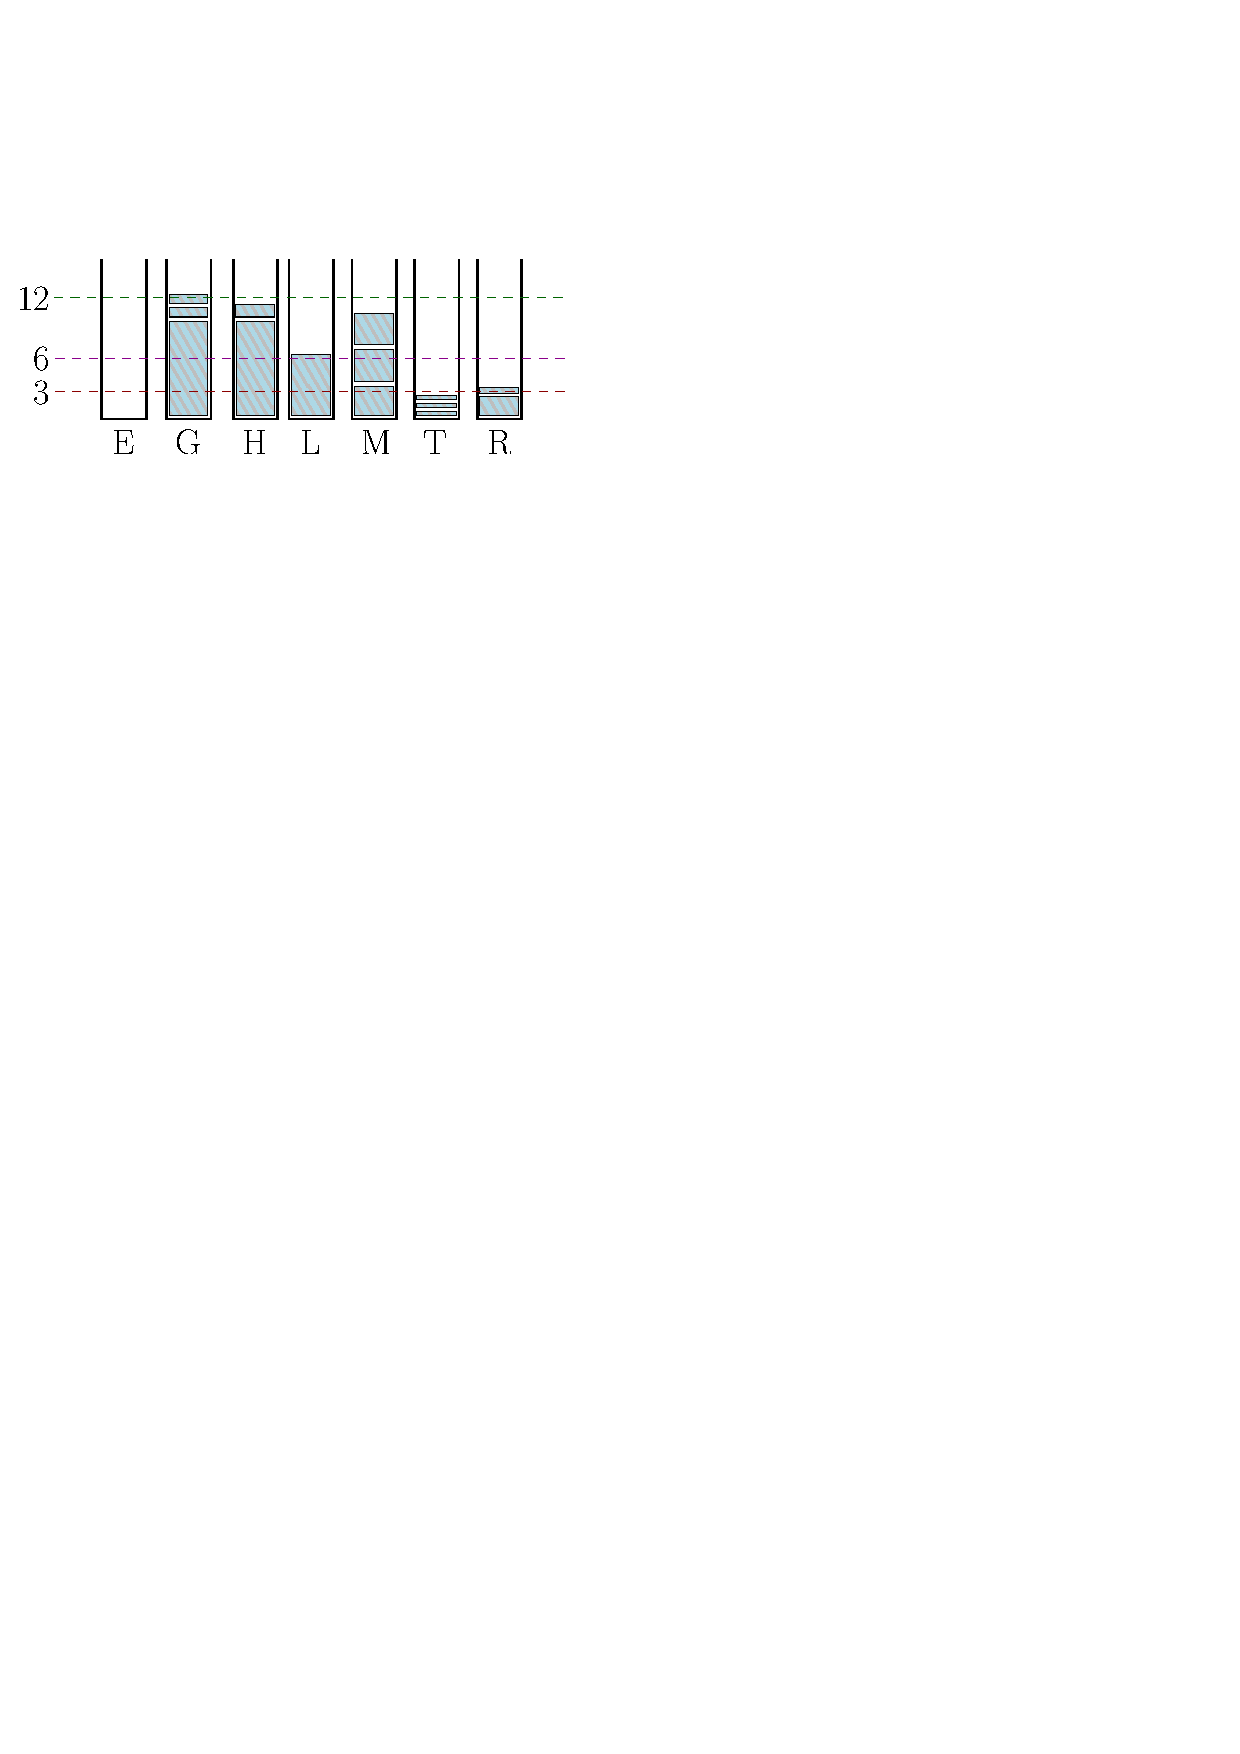
\includegraphics[width=0.7\textwidth]{img/bin_types.pdf}
\end{center}
\caption{An illustration of bin types during the first phase of our algorithm with stretching factor 1.5.}
\label{fig:1a}
\end{figure}
%

% \noindent{\bf First phase.}

\subsection{Classification of bins}

Along with items of specific types, we also wish to classify bins
based on which types of items they contain as well as other properties
(load, weight, value).

While item types are persistent, bin types change as items are added
to the bins. As mentioned, our algorithm will work in two phases, and
we make use of the bin types only during the first phase and when
transitioning into the second phase.

During the first phase, our algorithm maintains the invariant that
only bins of certain types exist, namely those from
Definition~\ref{d:types}. See Figure~\ref{fig:1a} for an illustration
of these types.

\begin{dfn}\label{d:types}
Given a bin $A$, we define the following bin types and introduce
letters that typically denote those bins:

\begin{compactitem}
\item 
{\bf Empty bins (E):} bins that have no item.
\item 
{\bf Complete bins (G):} all bins that have $w(A)\geq 0$ and $s(A)\geq
12$;
\item 
{\bf Huge-item bins (H):} all bins that contain a huge item (plus possibly some other items) and have $s(A)<12$;
\item 
{\bf One large-item bin (L):} a bin containing only a single large
item;
\item 
{\bf One medium-item bin (M):} a non-empty bin with $s(A)<13$ and only medium
items;
\item 
{\bf One tiny bin (T):} a non-empty bin with $s(A)\leq3$;
\item 
{\bf Regular bins (R):} all other bins with $s(A)\in(3,6]$;
\end{compactitem}
\end{dfn}



\section{First-phase algorithm}

During the algorithm, let $e$ be the current number of empty bins and
$r$ the current number of regular bins. 

\algobox{{\bf First-phase algorithm:}
\begin{compactenum}[(1)]
\item While $r < 3e$, consider the next item $i$ and pack it as
  follows, using bins of capacity 18; 
if more bins satisfy a condition, choose among them arbitrarily:
\item \indentskip If $i$ is regular:
\item \indentskip \indentskip If there is a huge-item bin, pack $i$ there.
\item \indentskip \indentskip Else, if there is a regular bin $A$ 
with $s(A)+s(i)\leq 6$, pack it there.
\item \indentskip \indentskip Else, if there is a tiny bin $A$
with $s(A)+s(i)\leq 6$, pack it there.
\item \indentskip If $i$ is medium and there is a medium-item bin where $i$ fits, pack it there.
\item \indentskip If $i$ is large and there is a large-item bin where $i$ fits, pack it there.
\item \indentskip If $i$ is huge:
\item \indentskip \indentskip If there is a regular bin, pack $i$ there.
\item \indentskip \indentskiptwodigit Else, if there is a tiny bin, pack $i$ there.
\item \indentskiptwodigit If $i$ is still not packed, pack it in an
  empty bin.
\end{compactenum}
}

First we observe that the algorithm above is properly defined.  The
stopping condition guarantees that the algorithm stops when no empty
bin is available. Thus an empty bin is always available and each item
$i$ is packed.  We now state the basic properties of the algorithm.

\begin{lem}
\label{l:1} 
At any time during the first phase the following holds:
\begin{compactenum}[\rm(i)]
\item 
\label{i1:classify} 
All bins used by the algorithm are of the types from Definition~\ref{d:types}.
\item 
\label{i1:complete} 
All complete bins $B$ have $v(B)\geq0$.
\item 
\label{i1:hr} 
If there is a huge-item bin, then there is no regular and no tiny bin.
\item 
\label{i1:lm} 
There is at most one large-item bin and at most one medium-item bin.
\item 
\label{i1:tiny} 
There is at most one tiny bin $T$. If $T$ exists, then for any regular
bin, $s(T)+s(R)>6$. There is at most one regular bin $R$ with
$s(R)\leq 4$.
\item 
\label{i1:er} 
At the end of the first phase $3e\leq r \leq 3e+3$.
\end{compactenum}
\end{lem}
\begin{proof}
(\ref{i1:classify})-(\ref{i1:tiny}): We verify that these invariants
  are preserved when an item of each type arrives and also that the
  resulting bin is of the required type; the second part is always
  trivial when packing in an empty bin.

If a huge item arrives and a regular bin exists, it always fits there,
thus no huge-item bin is created and (\ref{i1:hr}) cannot become
violated. Furthermore, the resulting size is more than $12$, thus the
resulting bin is complete. Otherwise, if a tiny bin exists, the huge
item fits there and the resulting bin is either complete or huge. In
either case, if the bin is complete, its value is 0 as it contains a
huge item.

If a large item arrives, it always fits in a large-item bin if it
exists and makes it complete; its value is at least 1, as it contains
two large items. Thus a second large-item bin is never
created and (\ref{i1:lm}) is not violated.

If a medium item arrives, it always fits in a medium-item bin if it
exists; the bin is then complete if it has size at least 13 and then
its value is at least 1, as it contains 4 or 5 medium items; otherwise
the bin type is unchanged. Again, a second medium-item bin is never
created and (\ref{i1:lm}) is not violated.

If a regular item arrives and a huge-item bin exists, it always fits
there, thus no regular bin is created and (\ref{i1:hr}) cannot become
violated. Furthermore, if the resulting size is at least $12$, the bin
becomes complete and its value is 0 as it contains a huge item; otherwise
the bin type is unchanged.

In the last case, a regular item arrives and no huge-item bin exists.
The algorithm guarantees that the resulting bin has size at most 6,
thus it is regular or tiny. We now proceed to verify
(\ref{i1:tiny}). A new tiny bin $T$ can be created only by packing an
item of size at most 3 in an empty bin. First, this implies that no
other tiny bin exists, as the item would be put there, thus there is
always at most one tiny bin. Second, as the item is not put in any
existing regular bin $R$, we have $s(R)+s(T)>6$ and this also holds
later when more items are packed into any of these bins. A new regular
bin $R$ with $s(R)\leq 4$ can be created only from a tiny bin; note
that a bin created from an empty bin by a regular item is either tiny
or has size in $(4,6]$. If another regular bin with size at most 4
  already exists, then both the size of the tiny bin and the size of
  the new item are larger than 2 and thus the new regular bin has size
  more than 4. This completes the proof of (\ref{i1:tiny}). 

(\ref{i1:er}): Before an item is packed, the value $3e-r$ is at least
  $1$ by the stopping condition. Packing an item may change $e$ or $r$ (or both) by at most $1$. Thus after
  packing an item we have $3e-r\geq 1-3-1=-3$, i.e., $r\leq 3e+3$. If
  in addition $3e\leq r$, the algorithm stops in the next step and
  (\ref{i1:er}) holds.  \qed
\end{proof}

\paragraph{Terminating the first phase. } If the algorithm packs all
input items in the first phase, it stops. Otherwise according to
Lemma~\ref{l:1}(\ref{i1:hr}) we split the algorithm in two very
different branches. If there is at least one huge-item bin, follow the
\emph{second phase with huge-item bins} below. If there is no huge-item bin,
we follow the \emph{second phase with regular bins}.

Any bin that is complete is not used in the second phase. In addition
to complete bins and either huge-item bins, or regular and empty bins,
there may exist at most three \emph{special bins} denoted and ordered
as follows: the large-item bin $L$, the medium-item bin $M$, and the
tiny bin $T$.


\section{Second phase with huge-item bins}
In this case, we assume that a huge-item bin exists when the first
phase ends. By Lemma~\ref{l:1}(\ref{i1:hr}), we know that no regular
and tiny bins exist. There are no empty bins either, as we end the
first phase with $3e \le r = 0$. With only a few types of bins
remaining, the algorithm for this phase is very simple:

\algobox{
{\bf Algorithm for the second phase with huge-item bins:}

Let the list of bins $\calL$ contain first all the huge-item bins,
followed by the special bins $L$, $M$, in this order, if they
exist.

\begin{compactenum}[(1)]
\item For any incoming item $i$:
\item \indentskip Pack $i$ using First Fit on the list $\calL$, with
  all bins of capacity 18. 
\end{compactenum}
}

Suppose that we have an instance that has a packing into bins of
capacity 12 and on which our algorithm fails. 
%
We may assume that the algorithm fails on the last item $f$.  By
considering the total volume, there always exists a bin with size at
most $12$. Thus $s(f)>6$ and $v(f)\ge2$.

If during the second phase an item $n$ with $s(n)\leq6$ is packed into
the last bin in $\calL$, we know that all other bins have size more
than $12$, thus all the remaining items fit into the last bin.
Otherwise we consider $v(\calL)$. Any complete bin $B$ has
$v(B)\geq0$ by Lemma~\ref{l:1}(\ref{i1:complete}) and each huge-item
bin gets nonnegative value, too. Also $v(L)\geq-1$ if $L$
exists. This shows that $M$ must exist, since otherwise
$v(\calL)+v(f)\geq-1+2\geq 1$, a contradiction.

Now we know that $M$ exists, furthermore it is the last bin and thus
we also know that no regular item is packed in $M$. Therefore $M$
contains only medium items from the first phase and possibly large
and/or huge items from the second phase. We claim that
$v(M)+v(f)\geq2$ using the fact that $f$ does not fit into $M$ and $M$
contains no item $a$ with $v(a)=0$: If $f$ is huge we have $s(M)>6$,
thus $M$ must contain either two medium items or at least one medium
item together with one large or huge item and $v(M)\geq -1$.  If $f$
is large, we have $s(M)>9$; thus $M$ contains either three medium
items or one medium and one large or huge item and $v(M)\geq 0$. Thus
we always have $v(\calL)\geq -1+v(M)+v(f)\geq 1$, a contradiction.


\section{Second phase with regular bins}

Let $\calE$ resp. $\calR$ be the set of empty resp. regular bins at
the beginning of the second phase, and let $e=|\calE|$. Let
$\lambda\in\{0,1,2,3\}$ be such that $|\calR|=3e+\lambda$;
Lemma~\ref{l:1}(\ref{i1:er}) implies that $\lambda$ exists. Note
that it is possible that $\calR=\emptyset$, in that case $e=\lambda=0$.

We organize the remaining non-complete bins into blocks $\calB_i$, and
then order them into a list $\calL$, as follows:

\begin{dfn}\label{d:blocks}
Denote the empty bins $E_1, E_2, \dots, E_e$.  The regular
bins are denoted by $R_{i,j}$, $i=1,...,e+1$, $j=1,2,3$. The $i$th
\textbf{block} $\calB_i$ consists of bins $R_{i,1},R_{i,2},R_{i,3},E_i$ in this
order. There are several modifications to this rule:
\begin{compactenum}[\rm (1)] 
\item The first block $\calB_1$ contains
only $\lambda$ regular bins, i.e., it contains $R_{1,1},\ldots,R_{1,\lambda},E_1$ in this
order; in particular, if $\lambda=0$ then $\calB_1$ contains only
$E_1$.

\item The last block $\calB_{e+1}$ has no empty bin,
only exactly $3$ regular bins. 

\item If $e=0$ and $r=\lambda>0$ we define only a single block $\calB_1$
which contains $r=\lambda$ regular bins $R_{1,1},\ldots,R_{1,\lambda}$. 

\item If $e=r=\lambda=0$, there is no block, as there are no empty and
  regular bins. 

\item  If $r>0$, we choose as the first regular bin the one with
size at most $4$, if there is such a bin. 
\end{compactenum}
Denote the first regular bin by $\Rbar$.  If no regular bin exists
(i.e., if $r=0$), $\Rbar$ is undefined.
\end{dfn}
Note that $\Rbar$ is either the first bin $R_{1,1}$ in $\calB_1$ if
$\lambda>0$ or the first bin $R_{2,1}$ in $\calB_2$ if $\lambda=0$. By
Lemma~\ref{l:1}(\ref{i1:tiny}) there exists at most one regular bin
with size at most $4$, thus all the remaining $R_{i,j}\neq\Rbar$ have
$s(R_{i,j})>4$.
\begin{dfn}\label{d:list}
The \textbf{list of bins} $\calL$ we use in the second phase contains first the
special bins and then all the blocks $\calB_1$, \ldots, $\calB_{e+1}$.
Thus the list $\calL$ is (some or all of the first six bins may not
exist):
\[
L, M, T, R_{1,1}, R_{1,2}, R_{1,3}, E_1, R_{2,1}, R_{2,2}, R_{2,3},
E_2, \dots,
E_e,  R_{e+1,1}, R_{e+1,2}, R_{e+1,3}.
\]
\end{dfn}
Whenever we refer to the ordering of the bins, we mean the ordering in
the list $\calL$. See Figure~\ref{fig:1} for an illustration.

\begin{figure}[th]
\begin{center}
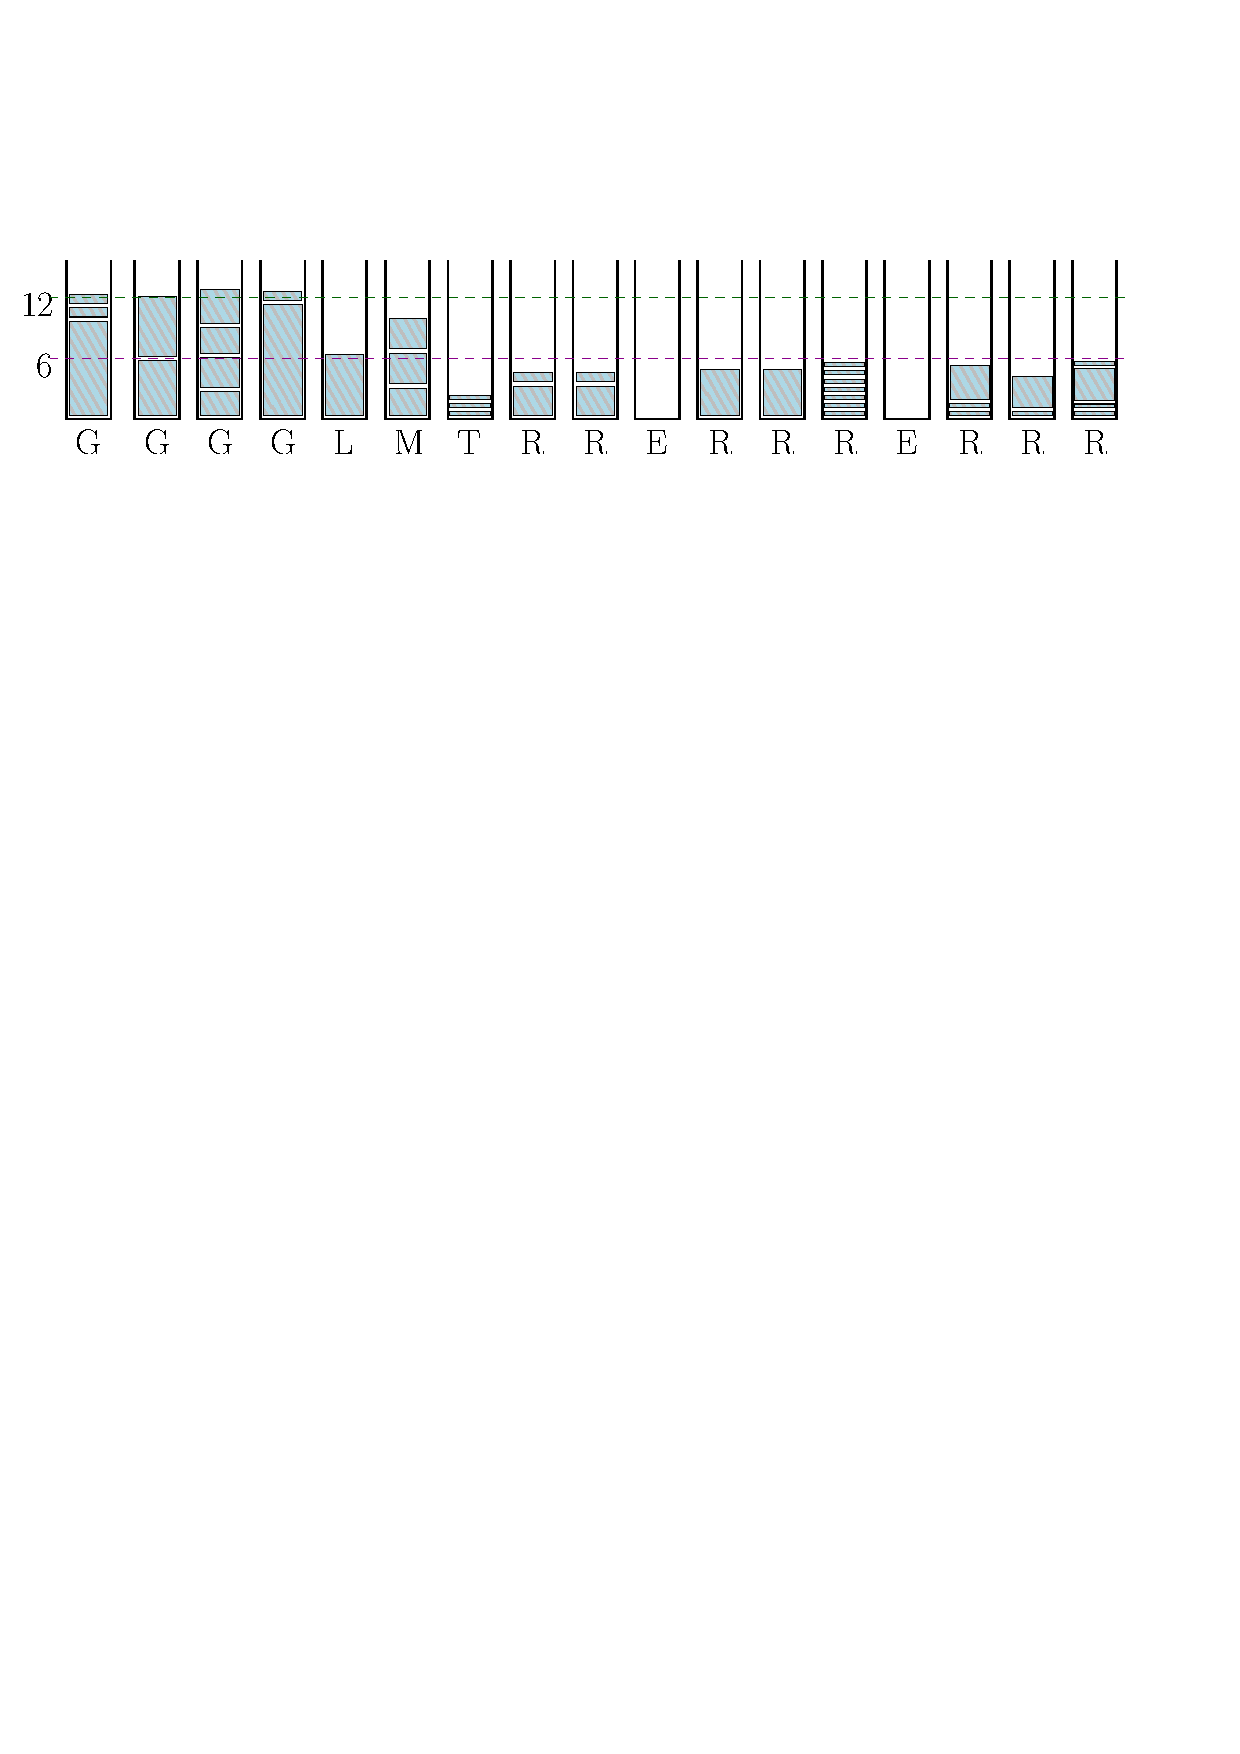
\includegraphics[width=\textwidth]{img/first_phase.pdf}
\end{center}
\caption[A typical state of the algorithm after the first phase.]{A typical state of the algorithm after the first phase. The bin labels correspond to the particular bin types. $G$ denotes complete bins, other labels are the initial letters of the bin types. The non-complete bins (other than $G$) are ordered as in
  the list $\calL$ at the beginning of the second phase with regular
  bins.}
\label{fig:1}
\end{figure}

\algobox{{\bf Algorithm for the second phase with regular bins:}

Let $\calL$ be the list of bins as in Definition~\ref{d:list}, with
all bins of capacity 18. 

\begin{compactenum}[(1)]

\item For any incoming item $i$:
\item \indentskip If $i$ is huge, pack it using First Fit on the
  reverse of the list $\calL$.
\item \indentskip In all other cases, pack $i$ using First Fit on the normal list $\calL$.
\end{compactenum}
}

Suppose that we have an instance that has a packing into bins of
capacity 12 and on which our algorithm fails. We may assume that the
algorithm fails on the last item. Let us denote this item by $f$.
We have $s(f)>6$, as otherwise all bins have size more than 12,
contradicting the existence of optimal packing.
Call the items that arrived in the second phase {\em new} (including
$f$), the items from the first phase are {\em old}.
See Figure~\ref{fig:2} for an illustration of a typical final
situation (and also of notions that we introduce later).

Our overall strategy is to obtain a contradiction by showing that  
$$w(\calL)+w(f)>0\,.$$ 
In some cases, we instead argue that
$v(\calL)+v(f)>0$ or $s(\calL)+s(f)>12|\calL|$. Any of these is
sufficient for a contradiction, as all complete bins have both
value and weight nonnegative and size at least 12.

Let $\calH$ denote all the bins from $\calL$ with a huge item,
and let $\hmodfour=|\calH| \bmod 4$. First
we show that the average size of bins in $\calH$ is large and exclude
some degenerate cases; in particular, we exclude the case when no
regular bin exists.

\begin{lem}
\label{l:huge} 
Let $\rho$ be the total size of old items
in $\Rbar$ if $\calR\neq\emptyset$ and $\Rbar\in\calH$, otherwise set $\rho=4$.
\begin{compactenum}[\rm (i)]
\item \label{i:hspecial} 
The bins $\calH$ are a final segment of the list $\calL$ and
$\calH\subsetneq\calE\cup\calR$. In particular, $\calR\neq\emptyset$
and $\Rbar$ is defined.
\item \label{i:hr}
We have
$s(\calH)\geq12|\calH|+\hmodfour+\rho-4$. 
\item \label{i:h}
If $\calH$ does not include $\Rbar$, then
$s(\calH)\geq12|\calH|+\hmodfour\geq12|\calH|$. 
\item \label{i:hfirst}
If $\calH$ includes $\Rbar$, then
$s(\calH)\geq12|\calH|+\hmodfour-1\geq12|\calH|-1$.
\end{compactenum} 
\end{lem}
\begin{proof}
First we make an easy observation used later in the proof. If
$\calE\cup\calR\cup\{T\}$ contains a bin $B$ with no huge item,
then no bin preceding $B$ contains a huge item.  Indeed, if a huge
item does not fit into $B$, then $B$ must contain a new item $i$ of
size at most $9$. This item $i$ was packed using First Fit on the
normal list $\calL$, and therefore it did not fit into any previous
bin. Thus the huge item also does not fit into any previous bin, and
cannot be packed there.

Let $\calH'=\calH\cap(\calE\cup\calR)$. We begin proving our lemma for
$\calH'$ in place of $\calH$.  That is, we ignore the special bins at
this stage. 
The previous observation shows that $\calH'$ is a final segment of the
list.

We now prove the claims (\ref{i:hr})--(\ref{i:hfirst}) with
$\calH'$ in place of $\calH$. 
All bins $R_{i,j}$ with a huge item have size at least $4+9=13$, with
a possible exception of $\Rbar$ which has size at least
$\rho+9=13+\rho-4$, by the definition of $\rho$. Each $E_i$ with a
huge item has size at least $9$. Thus for each $i$ with
$E_i\in\calH'$, $s(E_i)+s(R_{i+1,1})+s(R_{i+1,2})+s(R_{i+1,3})\geq
4\cdot 12$, with a possible exception of $i=1$ in the case when
$\lambda=0$. Summing over all $i$ with $E_i\in\calH'$ and the $\hmodfour$
bins in $\calR$ from the first block intersecting $\calH'$, and
adjusting for $\Rbar$ if $\Rbar\in\calH'$, (\ref{i:hr}) for $\calH'$
follows. The claims (\ref{i:h}) and (\ref{i:hfirst}) for $\calH'$ are
an immediate consequence as $\rho>3$ if $\Rbar\in\calH'$ and $\rho=4$
otherwise.

We claim that the lemma for $\calH$ follows if
$\calH'\subsetneq\calE\cup\calR$. Indeed, following the observation at
the beginning of the proof, the existence of a bin in $\calE\cup\calR$
with no huge item implies that no special bin has a huge item, i.e.,
$\calH'=\calH$, and also $\calH'=\calH$ is a final segment of
$\calL$. Furthermore, the existence of a bin in $\calE\cup\calR$
together with $3e\leq r$ implies that there exist at least one regular
bin, thus also $\Rbar$ is defined and (\ref{i:hspecial}) follows.
Claims (\ref{i:hr}), (\ref{i:h}), and (\ref{i:hfirst}) follow from
$\calH'=\calH$ and the fact that we have proved them for $\calH'$.

Thus it remains to show that $\calH'\subsetneq\calE\cup\calR$.
Suppose for a contradiction that $\calH'=\calE\cup\calR$.

If $T$ exists, let $o$ be the total size of old items in $T$. If also
$\Rbar$ exists, Lemma~\ref{l:1}(\ref{i1:tiny}) implies that
$o+\rho>6>4$, otherwise $o+\rho>4$ trivially. In either case, summing
with (\ref{i:hr}) we obtain
\begin{equation}\label{eq:Told}
  o+s(\calH')>12|\calH'|\,.
\end{equation}

Now we proceed to bound $s(\calH)$. We have already shown claim
(\ref{i:hfirst}) for $\calH'$, i.e., $s(\calH')\geq12|\calH'|-1$. If $L$ or
$M$ has a huge item, the size of the bin is at least 12, as there is
an old large or medium item in it. If $T$ has a huge item, then
(\ref{eq:Told}) implies $s(T)+s(\calH')>9+
o+s(\calH')>9+12|\calH'|$. Summing these bounds we obtain

\begin{equation}
s(\calH) > 12|\calH|-3 \,. \label{eq:T}
\end{equation}
 
We now derive a contradiction in each of the following four cases.

\mycase{Case 1:} All special bins have a huge item.  Then
$\calL=\calH$ and (\ref{eq:T}) together with $s(f)>6$ implies
$s(\calL)+s(f)>12|\calL|+3$, a contradiction.

\mycase{Case 2:} There is one special bin with no huge item.  Then its
size together with $f$ is more than 18, thus (\ref{eq:T}) together
with $s(f)>6$ implies $s(f)+s(\calL)>18+12|\calH|-3>12|\calL|$, a
contradiction.

\mycase{Case 3:} There are two special bins with no huge item and these
bins are $L$ and $M$.

Suppose first that $M$ contains a new item $n$. Then $s(L)+s(n)>18$ by
the First Fit packing rule. The bin $M$ contains at least one old
medium item.  Thus, using (\ref{eq:T}), we get
$s(f)+s(\calL)>6+s(L)+s(n)+3+12|\calH|-3> 24+ 12|\calH|=12|\calL|$, a
contradiction.

If $M$ has no new item, then either $f$ is huge and $M$ has at least
two medium items, or $f$ is large and $M$ has at least three items. In
both cases $v(M)+v(f)\geq 2$. Also $v(L)\geq -1$ since $L$ has a large
item, and $v(\calH)\geq0$ as each bin has a huge item. Altogether we
get that the total value $v(\calL)>0$, a contradiction.

\mycase{Case 4:} There are two or three special bins with no huge
item, one of them is $T$. Observe that the bin $T$ always contains a
new item $n$, as the total size of all old items in it is at most $3$. 

If there are two special bins with no huge item, denote the first one by
$B$. As we observed at the beginning of the proof, if $T$ exists and
has no huge item, no special bin can contain a huge item, thus the
third special bin cannot exist. We have
$s(B)+s(n)>18$, summing with (\ref{eq:Told}) we obtain
$s(f)+s(\calL)\geq
s(f)+s(B)+s(n)+o+s(\calH')>6+18+12|\calH'|=12|\calL|$, a contradiction.

If there are three special bins with no huge item, we have
$s(f)+s(L)>18$ and $s(M)+s(n)>18$. Summing with (\ref{eq:Told}) we
obtain $s(f)+s(\calL)>18+18+o+s(\calH')>36+12|\calH'|=12|\calL|$, a
contradiction.
%\qed
\end{proof}

Having proven Lemma~\ref{l:huge}, we can infer existence of the following
two important bins, which (as we will later see) split the instance into three
logical blocks:

\begin{dfn} ~ 

\begin{compactitem} \label{d:fc}
\item Let $F$, the \textbf{final bin} be the last bin in $\calL$ before
$\calH$, or the last bin if $\calH=\emptyset$.
\item Let $C$, the \textbf{critical bin}, be the
first bin in $\calL$ of size at most 12. 
\end{compactitem}
\end{dfn}

First note that both $F$ and $C$ must exist: $F$ exists by
Lemma~\ref{l:huge}(\ref{i:hspecial}), which also shows that
$F\in\calE\cup\calR$. $C$ exists, as otherwise the total size is more
than $12m$.

To make our calculations easier, we modify the packing so that $f$ is put
into $F$, even though it exceeds the capacity of $F$.
Thus $s(F)>18$ and $f$ (a new item) as well as all the other new items packed
in $F$ or in some bin before $F$ satisfy the property that they do not
fit into any previous bin.  See Figure~\ref{fig:2} for an illustration
of the definitions.

We start by some easy observations. Each bin, possibly with the
exception of $L$ and $M$, contains a new item, as it enters the phase
with size at most 6, and the algorithm failed. Only items of size at
most $9$ are packed in bins before $F$; in $F$ itself only the item
$f$ can be huge.  The bin $F$ always has at least two new items, one that did
fit into it and $f$. All the new items in the bins after $C$ are
large, except for the new huge items in $\calH$ and $f$ which can be
large or huge. (Note that at this point of the proof it is possible
that $C$ is after $F$; we will exclude this possibility soon.)

\begin{figure}[th]
\begin{center}
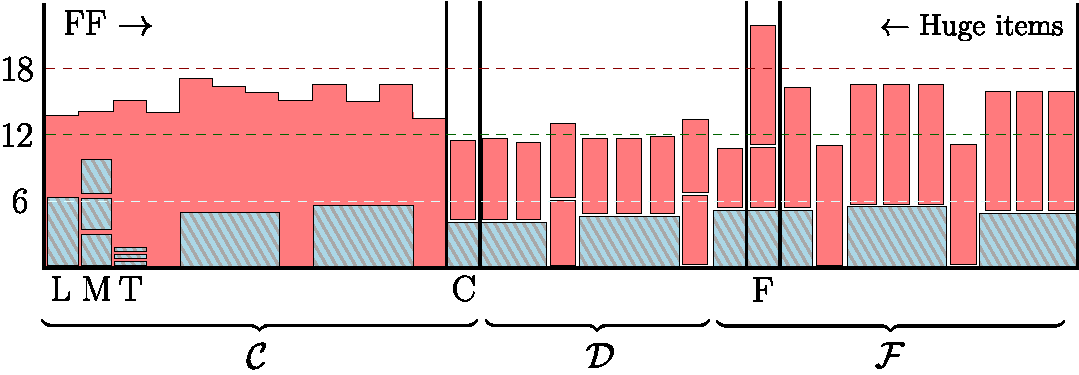
\includegraphics[width=1\textwidth]{img/second_phase.pdf}
\end{center}
\caption[A typical state of the algorithm after the second phase
with regular bins.]{A typical state of the algorithm after the second phase with regular
  bins. The gray (hatched) areas denote the old items (i.e., packed in
  the first phase), the red (solid) regions and rectangles denote the
  new items (i.e., packed in the second phase). The bins that are
  complete at the end of the first phase are not shown. The item $f$
  on which the algorithm fails is shown as packed into the final bin
  $F$ and exceeding the capacity $18$, following the convention
  introduced after Definition~\ref{d:fc}.}
\label{fig:2}
\end{figure}

More observations are given in the next two lemmata.

\begin{lem}
\label{l:aux}
\begin{compactenum}[(i)]
\item
\label{i:9}
Let $B$ be any bin before $F$. Then $s(B)>9$. Furthermore, if
$B\in\calE$ then $B$ contains at least two new items.
\item
\label{i:12}
Let $B,B',B''$ be any three bins in the ordering $\calL$ with
$B <_{\calL} B' <_{\calL} B'' \leq_{\calL} F$ and let $B''$ contain at least two new items. Then
$s(B)+s(B')+s(B'')>36+o$, where $o$ is the size of old items in $B''$.
\item  
\label{i:11}
Let $B$ be arbitrary and let $B'\in\calR$ be a bin such that $B <_{\calL} B' \leq_{\calL} F$.

If $B'\neq\Rbar$ then $s(B)+s(B')>22$, in
particular $s(B)>11$ or $s(B')>11$.

If $B'=\Rbar$ then $s(B)+s(B')>21$.
\end{compactenum}
\end{lem}

\begin{proof}
$F$ contains a new item $n$ different from $f$. To prove (\ref{i:9}),
  note that $s(n)\leq 9$, and $n$ does not fit into $B$. It follows
  that if $B\in\calE$, then $B$ must contain at least two new items,
  as only items with size smaller than $9$ are packed before $F$.

To prove (\ref{i:12}), let $n,n'$ be two new items in $B''$ and note
that $s(B)+s(n)>18$ and $s(B')+s(n')>18$.

To prove (\ref{i:11}), observe that $B'$ has a new
item of size larger than $18-s(B)$, and it also has old items of size
at least $3$ or even $4$ if $B'\neq\Rbar$.
% \qed
\end{proof}

\begin{lem}
\label{l:cf} 
The critical bin $C$ is before $F$, there are at least two bins
between $C$ and $F$ and $C$ is not in the same block as $F$.
\end{lem}
\begin{proof}
All bins before $C$ have size larger than $12$. Using
Lemma~\ref{l:huge} we have
$$s(F)+s(\calH)>18+12|\calH|-1=12(|\calH|+1)+5\,.$$ 
It remains to bound the sizes of the other bins. Note that $F\neq C$ as $s(F)>18$.
If $C$ is after $F$,
all bins before $F$ have size more than $12$, so all together
$s(\calL)>12|\calL|+5$, a contradiction. If $C$ is just before $F$,
then by Lemma~\ref{l:aux}(\ref{i:9}),
$s(C)>9=12-3$ and the total size of bins in $s(\calL)>
12|\calL|+5-3>12|\calL|$, a contradiction.

If there is a single bin $B$ between $C$ and $F$, then $s(C)+s(B)$
plus the size of two new items in $F$ is more than $36$ by
Lemma~\ref{l:aux}(\ref{i:12}). If $F\in\calE$ then $\calH$ starts with
three bins in $\calR$, thus $s(\calH)\geq12|\calH|+2$ using 
Lemma~\ref{l:huge} with $\hmodfour=3$, and we get a
contradiction. If $F\in\calR$ then $\Rbar\notin\calH$, thus
Lemma~\ref{l:huge} gives $s(\calH)\geq12|\calH|$, and we get a
contradiction as well.

The last case is when $C$ and $F$ are in the same block with two bins
between them. Then $F\in\calE$, so $\hmodfour=3$, and $C$ is the first
bin of the three other 
bins from the same block, so $\Rbar\notin\calH$. Then $s(C)>9$, the
remaining two bins together with $F$ have size more than $36$ by
Lemma~\ref{l:aux}(\ref{i:12}) and we use $s(\calH)\ge 12|\calH|+3$ from
Lemma~\ref{l:huge} to get a contradiction.
% \qed
\end{proof}
We now partition $\calL$ into several parts (see Figure~\ref{fig:2} for an illustration):

\begin{dfn}~
\begin{compactitem}
\item Let $\calF=\calB_i\cup\calH$, where $F\in\calB_i$.
\item Let $\calD$ be the set of all bins after $C$ and before $\calF$.
\item Let $\calC$ be the set of all bins before and including $C$.
\end{compactitem}
\end{dfn}

Lemma~\ref{l:cf} shows that the
parts are non-overlapping. We analyze the weight of the parts
separately, essentially block by block.
Recall that a weight of a bin is defined as $w(A)=s(A)+k(A)-13$,
where $k(A)$ is the number of large and huge items packed in $A$.
The proof is relatively
straightforward if $C$ is not special (and thus also
$F\not\in\calB_1$), 
which is the most important case driving our choices for $w$. 
A typical block has nonnegative weight, we gain more
weight in the block of $F$ which exactly compensates the loss of
weight in $\calC$, which occurs mainly in $C$ itself. 

Let us formalize and prove the intuition stated in the previous
paragraph in a series of three lemmata.

\begin{lem}
\label{l:f} 
If $F$ is not in the first block then $w(\calF)>5$, otherwise $w(\calF)>4$.
\end{lem}
\begin{proof}
All the new items in bins of $\calF$ are large or huge. Each bin has a
new item and the bin $F$ has two new items. Thus $k(\calF)\geq
|\calF|+1$. All that remains is to show that $s(\calF)>12|\calF|+3$,
and $s(\calF)>12|\calF|+4$ if $F$ is not in the first block.

If $F$ is the first bin in a block, the lemma follows as $s(F)>18$ and
$s(\calH)\geq12|\calH|-1$, thus $s(\calF)=s(F)+s(\calH)>12|\calF|+5$.

In the remaining cases there is a bin in $\calR\cap\calF$ before $F$.
Lemma~\ref{l:huge} gives $s(\calH)\geq12|\calH|$; moreover, if
$F\in\calE$, then $s(\calH)\geq12|\calH|+3$.

If $F$ is preceded by three bins from $\calF\cap\calR$, then
$F\in\calE$ and thus $s(\calH)\geq12|\calH|+3$. Using
Lemma~\ref{l:aux}(\ref{i:11}) twice, two of the bins in
$\calF\cap\calR$ before $F$
have size at least $11$ and using Lemma~\ref{l:aux}(\ref{i:9}) the
remaining one has size $9$. Thus the size of these four bins is more
than $11+11+9+18=4\cdot12+1$, summing with the bound for $\calH$ we get
$s(\calF)>12|\calF|+4$. 

If $F$ is preceded by two bins from $\calF\cap\calR$, then by
Lemma~\ref{l:aux}(\ref{i:9}) the total size of these two bins and two
new items in $F$ is more than $36$. If $F\in\calR$, the size of old
items in $F$ is at least $4$ and with $s(\calH)\geq12|\calH|$ we get
$s(\calF)>12|\calF|+4$. 
If $F\in\calE$, which also implies that $F$ is in the first block, then
$s(\calH)\geq12|\calH|+3$, thus $s(\calF)>12|\calF|+3$. 

If $F$ is preceded by one bin $R$ from $\calF\cap\calR$, then let $n$ be a
new item in $F$ different from $f$. We have $s(R)+s(n)>18$ and
$s(f)>6$. We conclude the proof as in the previous case.
% \qed
\end{proof}

\begin{lem}
\label{l:c} ~

If $C\in\calR$ then $w(\calC)\geq -6$. 

If $C\in\calE$ then $w(\calC)\geq -5$. 

If $C$ is a special bin then $w(\calC)\geq -4$.
\end{lem}

\begin{proof}
For every bin $B$ before $C$, $s(B)>12$ and thus $w(B)>-1$ by the
definition of $C$. Let $\Cprime$ be the set of all bins $B$ before $C$ with
$w(B)\leq0$. This implies that for $B\in\Cprime$, $s(B)\in(12,13]$
and $B$ has no large item. It follows that any new item in any
bin after the first bin in $\Cprime$ has size more than $5$.
We have 
\begin{equation}
\label{eq:wcalC}
w(\calC)\geq w(\Cprime)+w(C)\geq-|\Cprime|+w(C)\,.
\end{equation} 

First we argue that either $|\Cprime|\leq 1$ or $\Cprime=\{M,T\}$.
Suppose that $|\Cprime|>1$, choose $B,B'\in\Cprime$ so that $B$ is before
$B'$.  If $B'\in\calE$, either $B'$ has at most two (new) non-large items and
$s(B')\leq 6+6= 12$, or it has at least three items and
$s(B')>5+5+5=15$; both options are impossible for $B'\in\Cprime$.
If $B'\in\calR$, it has old items of total size in
$(3,6]$. Either $B'$ has a single new item and $s(B')\leq 6+6= 12$, or
it has at least two new items and $s(B')>3+5+5=13$; both options
are impossible for $B'\in \Cprime$. 
The only remaining
option is that $B'$ is a special bin. Since $L$ has a large item,
$L\not\in\Cprime$ and $\Cprime=\{M,T\}$.

By Lemma~\ref{l:aux}(\ref{i:9}), we have $w(C)\geq -4$. The lemma
follows by summing with (\ref{eq:wcalC}) in the following three cases: (i)
$C\in\calR$, (ii) if $\Cprime=\emptyset$ and also (iii) if
both $C\in\calE$ and $|\Cprime|=1$.

For the remaining cases, (\ref{eq:wcalC}) implies that it is
sufficient to show $w(C)\geq -3$. 
If $C\in\calE$ and $\Cprime=\{M,T\}$ then $C$ contains two new items of
size at least 5, thus $w(C)\geq -3$.
%
If $C=T$ and $\Cprime=\{M\}$ then $C$ either has a large item, or it
has two new items: otherwise it would have size at most 3 of old items
plus at most 6 from a single new item, total of at most 9,
contradicting Lemma~\ref{l:aux}(\ref{i:9}). Thus $w(C)\geq -3$ in this
case as well.
% \qed
\end{proof}

\begin{lem}
\label{l:d} 
\begin{compactenum}[\rm(i)]
\item 
For every block $\calB_i\subseteq\calD$ we have $w(\calB_i)\geq 0$.
\item 
If there is no special bin in $\calD$, then $w(\calD)\geq 0$.
If also $C\in\calR$ then $w(\calD)\geq 1$.
\end{compactenum}
\end{lem}

\begin{proof}
First we claim that for each block $\calB_i\subseteq\calD$ with three
bins in $\calR$, we have 
\begin{equation}
\label{eq:wB0}
w(\calB_i)\geq 0\,.
\end{equation} 
By Lemma~\ref{l:aux}(\ref{i:11}), one of the bins in $\calR\cap\calB_i$
has size at least 11. By Lemma~\ref{l:aux}(\ref{i:12}), the remaining
three bins have size at least 36. We get (\ref{eq:wB0}) by observing that
$k(\calB_i)\geq 5$, as all the new items placed after $C$ and
before $F$ are large, each bin
contains a new item and $E_i$ contains two new items.

Next, we consider an incomplete block, that is,
a set of bins $\calB$ with at most two bins
from $\calR\cap\calD$ followed by a bin $E\in\calE\cap\calD$.
We claim 
\begin{equation}
\label{eq:wcalB}
w(\calB)\geq 1\,. 
\end{equation}
The bin $E$ contains two large items, since it is after $C$. In particular,
$w(E)\geq 1$ and (\ref{eq:wcalB}) follows if $|\calB|=1$. If $|\calB|=2$, the
size of one item from $E$ plus the previous bin is more than 18, the
size of the other item is more than 6, thus $s(\calB)\geq 24$; since
$k(B)\geq 3$, (\ref{eq:wcalB}) follows.  If $|\calB|=3$, by
Lemma~\ref{l:aux}(\ref{i:12}) we have $s(\calB)\geq 36$; $k(\calB)\geq
4$ and (\ref{eq:wcalB}) follows as well.

By definition, $\calD$ ends by a bin in $\calE$ (if nonempty). Thus
the lemma follows by using (\ref{eq:wcalB}) for the incomplete block,
i.e., for $C\in\calR$ or for $\calB_1$ if it does not have three bins
in $\calR$, and adding (\ref{eq:wB0}) for all the remaining blocks.
Note that $C\in\calR$ implies $\calD\not=\emptyset$.
% \qed
\end{proof}

We are now ready to derive the final contradiction. 

If $\calD$ does not contain a special bin, we add the
appropriate bounds from Lemmata~\ref{l:c}, \ref{l:d} and~\ref{l:f}.
If $C\in\calR$ then $F$ is not in the first block and
$w(\calL)=w(\calC)+w(\calD)+w(\calF)>-6+1+5=0$.  If $C\in\calE$ then
$F$ is not in the first block and
$w(\calL)=w(\calC)+w(\calD)+w(\calF)>-5+0+5=0$.  If $C$ is the last
special bin then $w(\calL)=w(\calC)+w(\calD)+w(\calF)>-4+0+4=0$. In
all subcases $w(\calL)>0$, a contradiction.

The rest of the proof deals with the remaining case when $\calD$ does
contain a special bin. This implies there are at least two special
bins and $C$ is not the last special bin. Since $T$ is always the last
special bin (if it exists), it must be the case that $C\neq T$ and
thus $C=L$ or $C=M$.  We analyze the special bins together with the
first block, up to $F$ if $F$ belongs to it.  First observe that the
only bin possibly before $C$ is $L$ and in that case $w(L)\ge0$, so
$w(\calC)\geq w(C)$.

Let $A$ denote $F$ if $F\in\calB_1$ or $E_1$ if $F\not\in\calB_1$.  As
$A=F$ or $A\in\calE$, we know that $A$ contains at least two new
items; denote two of these new items by $n$ and $n'$. Since $A$ is
after $C$, we know that both $n$ and $n'$ are large or huge.

Let $\calA$ be the set
containing $C$ and all bins between $C$ and $A$, not including
$A$. Thus $\calA$ contains two or three special bins followed by at
most three bins from $\calR$. We have $k(\calA)\geq|\calA|-1$ as each
bin in $\calA$ contains a large item, with a possible exception of
$C$ (if $C=M$).  Furthermore $k(A)\geq2$. The bound on $k(\calA)$ and
$k(A)$ imply that
\begin{equation}
\label{eq:ws}
w(\calA)+w(A)\geq s(\calA)+s(A)-12|\calA|-12   
\end{equation}
and thus it is sufficient to bound $s(\calA)+s(A)$. 

The precise bound we need depends on what bin $A$ is.  In each case,
we first determine a sufficient bound on $s(\calA)+s(A)$ and argue
that it implies contradiction. Afterwards we prove the bound.
Typically, we bound the size by creating pairs of bins of size $21$ or
$22$ by Lemma~\ref{l:aux}(\ref{i:11}). We also use that $s(B)>9$ for
any $B\in\calA$ by Lemma~\ref{l:aux}(\ref{i:9}) and that $n$, $n'$
together with any two bins in $\calA$ have size at least $36$ by
Lemma~\ref{l:aux}(\ref{i:12}).

\mycasesp{Case $A\neq F$:} 
Then $F\not\in\calB_1$ and $A=E_1$. We claim that 
\begin{equation}
\label{eq:AneqF}
s(\calA)+s(A)\geq12|\calA|+7\,.
\end{equation}
First we show that~(\ref{eq:AneqF}) implies a contradiction. Indeed, 
(\ref{eq:AneqF}) together with (\ref{eq:ws}) yields
$w(\calA)+w(A)\geq -5$ and summing this with all the other bounds,
namely $w(\calF)>5$ from Lemma~\ref{l:f} and $w(\calB_i)\ge0$ for
whole blocks $\calB_i\in\calD$ from Lemma~\ref{l:d}, leads to
$w(\calL)>0$, which is a contradiction.  

Now we prove~(\ref{eq:AneqF}). The items $n$ and $n'$ from $A$
together with the first two special bins in $\calA$ have size more
than 36. Let $\Aprime$ be the set of the remaining bins; it contains
possibly $T$ and at most three bins from $\calR$.  It remains to show
$s(\Aprime)\geq 12|\Aprime|-5$.

For $|\Aprime|=0$ it holds trivially.  

If $|\Aprime|=1$, the only bin in $\Aprime$ has size more than
9 and this is sufficient. 

For $|\Aprime|>1$ we apply Lemma~\ref{l:aux}(\ref{i:11}) and pair as
many bins from $\Aprime$ as possible; note that all the bins in
$\Aprime$ except possibly $T$ are in $\calR$, so the assumptions of
the lemma hold.  If $|\Aprime|=2$, then
$s(\Aprime)>21=2\cdot12-3$. For $|\Aprime|=3$ we get
$s(\Aprime)>22+9=3\cdot12-5$, since we can create a pair without
$\Rbar$.  Finally, if $|\Aprime|=4$ then $s(\Aprime)>22+21=4\cdot
12-5$.

\mycasesp{Case $A=F$:} 
We claim that it is sufficient to prove
\begin{equation}
\label{eq:AF}
s(\calA)+s(n)+s(n')>12|\calA|+\begin{cases}
8 & \mbox{if $F\in\calR$ and $\Rbar\in\calA$,} \\
9 & \mbox{if either $F\in\calR$ or $\Rbar\in\calA$,} \\
10 & \mbox{in all cases.}
\end{cases}
\end{equation}
First we show that~(\ref{eq:AneqF}) implies a contradiction. 
 
If $F=E_1$ we note that $\hmodfour=3$ (as $\calH$ starts with $3$ bins
in $\calR$). Thus Lemma~\ref{l:huge}, items (\ref{i:h}) and
(\ref{i:hfirst}), together with $w(\calH)\geq s(\calH)-12|\calH|$
yields $w(\calH)\geq 3$ for $\Rbar\in\calA$ or $w(\calH)\geq 2$ for
$\Rbar\not\in\calA$. Summing this with $w(\calA)+w(A)>-3$ or
$w(\calA)+w(A)>-2$, that are obtained from (\ref{eq:ws}) and
(\ref{eq:AF}) in the respective cases, we obtain $w(\calL)>0$, a
contradiction.

If $F\in\calR$ then we know that $F$ also contains old items
of size at least 3 if $\Rbar\not\in\calA$ or even 4 if $\Rbar\in\calA$
(and thus $F\neq\Rbar$). Summing this with the respective bound from
(\ref{eq:AF}) we obtain $s(\calA)+s(F)>12|\calA|+12$. Summing this
with $s(\calH)\geq 12|\calH|$ from Lemma~\ref{l:huge}(\ref{i:h}) now
yields $s(\calL)>12|\calL|$, a contradiction.

Thus~(\ref{eq:AneqF}) always leads to a contradiction. 

We now distinguish subcases depending on $|\calA|$ and in each case we
either prove~(\ref{eq:AF}) or obtain a contradiction directly. 
Note that $\Rbar\in\calA$ whenever $|\calA|\geq 4$. 

\mycasesp{Case $|\calA|=2$:} The two bins together with $n$ and
$n'$ have size more than $36$. Thus
$s(\calA)+s(n)+s(n')>36=12\cdot2+12$, which implies~(\ref{eq:AF}). 

\mycasesp{Case $|\calA|=3$:} We have $s(C)>9$ and the remaining two
bins together with $n$ and $n'$ have size more than $36$. Thus
$s(\calA)+s(n)+s(n')>12|\calA|+9$, which implies~(\ref{eq:AF}) in all
cases except if $F=E_1$ and $\Rbar\not\in\calA$.  

In the remaining case, $\calA=\{L,M,T\}$ and $C=L$, as $\calA$
contains no bin from $\calR$ and $|\calA|=3$.  We prove a
contradiction directly. Let $o$ be the size of old items in $T$.  We
apply Lemma~\ref{l:huge}(\ref{i:hr}), using the fact that $o+\rho>6$
by Lemma~\ref{l:1}(\ref{i1:tiny}), where $\rho$ is the total size of
old items in $\Rbar\in\calH$, and $\hmodfour=3$. We get
$o+s(\calH)\geq o+12|\calH|+\hmodfour+\rho-4>12|\calH|+5$.  Let $n''$
be a new item in $T$. Since $n''$ does not fit into $M$,
$s(M)+s(n'')>18$; also $s(L)>9$ and $s(F)>18$. Summing all the bounds,
we have $s(\calL)\geq o+s(\calH)+s(M)+s(n'')+s(L)+s(F)
>12|\calH|+5+18+9+18=12|\calL|+2$, a contradiction.

\mycasesp{Case $|\calA|=4$:}
The last bin $R\in\calA$ is in
$\calR$. Together with any previous bin it has size more than $21$,
the remaining two bins together with $n$ and $n'$ have size more than
$36$ by Lemma~\ref{l:aux}(\ref{i:12}). 
Thus $s(\calA)+s(n)+s(n')>21+36=4\cdot12+9$ which implies~(\ref{eq:AF}),
since $\Rbar\in\calA$.

\mycasesp{Case $|\calA|=5$:}
First consider the case $F=E_1$. 
The last two bins of $\calA$ are in $\calR$, we pair
them with two previous bins to form pairs of size more than $21 + 22$.
The remaining bin has size at least $9$,
since $n$ does not fit into it and $s(n)<9$. We also have
$s(F)>18$. Thus $s(\calA)+s(A)>21+22+9+18=5\cdot12+10$, which
implies~(\ref{eq:AF}).

If $F\in\calR$ then one of the last two bins of $\calA$ has size more
than $11$ and the other forms a pair of size more than $21$ with one
special bin. The remaining two bins together with $n$ and $n'$ have
size more than 36 by Lemma~\ref{l:aux}(\ref{i:12}). Thus
$s(\calA)+s(n)+s(n')>11+21+36=5\cdot12+8$ which implies~(\ref{eq:AF}),
because $\Rbar\in\calA$.

\mycasesp{Case $|\calA|=6$:} Then $\calA$ contains all three special
bins and three bins from $\calR$, therefore also $F=E_1$. We form
three pairs of a special bin with a bin from $\calR$ of total size
more than $21+22+22$. Since $s(F)>18$, we have
$s(\calA)+s(F)>21+22+22+18=6\cdot12+11$.  Since in this case
$A=F=E_1$, we have $s(\calH)\geq 12|\calH|+3$ and
$s(\calL)>12|\calL|$, a contradiction.

In all of the cases we can derive a contradiction, which implies
that our algorithm cannot fail. This concludes the proof of
Theorem~\ref{thm:onepointfive}. \qed
\section{Tightness of the analysis}

We note that the analysis of our algorithm is tight, i.e., if we
reduce the capacity of the bins below 18, the algorithm
fails. Consider the following instance. Send two items of size 6
which are in the first phase packed separately into two bins. Then
send $m-1$ items of size 12. One of them must be put into a bin
with an item of size 6, i.e., one bin receives items of size 18, while
all the items can be packed into $m$ bins of size 12.

To decrease the upper bound below $1.5$ seems challenging. In
particular, the instance above and its modifications with more items
of size 6 or slightly smaller items at the beginning shows that these
items need to be packed in pairs. This in turns creates difficulties
that, in the current approach, lead to new item and bin types; at this
point we do not know if such an approach is feasible.

% Another possible research direction is to improve the lower bounds, in
% particular for large $m$. It is quite surprising that there are no
% lower bounds for $m>5$ larger than the easy bound of $4/3$.

% \noindent{\bf Acknowledgment.} The authors thank Emese Bittner for
% useful discussions during her visit to Charles University. We also
% thank to referees for many useful comments.

\openright\chapter{An Algorithm Fine-Tuned for Three Bins}
\label{chap:threebins}
% \addcontentsline{toc}{chapter}{Algorithms Fine-Tuned for Three Bins}

In this section, we focus on instances with exactly three bins. 
We prove the following:

\begin{thm}\label{thm:3binsalgo}
There exists an algorithm that solves
\binstretch for three bins with stretching factor $1+3/8=1.375$.
\end{thm}

Our final online algorithm uses several subroutines, one of which is
the classical online algorithm \FF:

\smallskip
\algobox{
\textbf{Subroutine \FF:}
\begin{compactenum}[(1)]
\item Set an ordering of your bins. 
\item For every incoming item $i$:
\item \indentskip Pack $i$ into the first bin where $i$ fits below or to the limit $t$.
\item \indentskip If no such bin exists, report failure.
\end{compactenum}
}
\smallskip

The three bins of our setting are named $A$, $B$, and $C$.  We
exchange the names of bins sometimes during the course of the
algorithm.

Throughout the proof, we will need to argue about loads of the bins
$A$, $B$, $C$ before various items arrived. The following notation
will help us in this endeavour:

Suppose that $A$ is a bin and $x$ is an item that gets packed at some
point of the algorithm (not necessarily into $A$).  Then $A_{\before
x}$ will indicate the set of items that are packed into $A$ just
before $x$ arrived.

We scale the input sizes by $16$. The stretched bins in our setting
therefore have capacity $22$ and the optimal offline algorithm can
pack all items into three bins of capacity $16$ each.

\section{Algorithm overview}\label{sec:3:algoverview}

If we were to design a new algorithm from scratch, we would probably
start with trying to pack first all items in a single bin, as long as
possible. In general, this is the strategy that the final algorithm
will also follow. However, somewhat surprisingly, it turns out that
from the very beginning we need to put items in two bins even if the
items as well as their total size are relatively small.

It is clear that we have to be very cautious about exceeding a load of
6. For instance, if we put 7 items of size 1 in bin $A$, and 7 such items in $B$,
then if two items of size 16 arrive, the algorithm will have a load of 
at least 23 in some bin. Similarly, we cannot assign too much to a single bin:
putting 20 items of size 0.5 all in bin $A$ gives a load of 22.5 somewhere if 
three items of size 12.5 arrive next. (Starting with items of size 0.5
guarantees that there is an optimal solution with bins of capacity 16.) 

On the other hand, it is useful to keep one bin empty for some time; many
problematic instances end with three large items such that one of them has
to be placed in a bin that already has high load. Keeping one bin free ensures
that such items must have size more than 11 (on average), which limits the
adversary's options, since all items must still fit into bins of size 16.

Deciding when exactly to start using the third bin and when to cross the
threshold of 6 for the first time was the biggest challenge in designing
this algorithm: both of these events should preferably be postponed as long
as possible, but obviously they come into conflict at some point.


\section{Good situations}\label{sec:3:gs}
Before stating the algorithm itself, we list a number of \textit{good
situations} (GS). These are configurations of the three bins which
allow us to complete the packing regardless of the following input.

It is clear that the identities of the bins are not important here;
for instance, in the first good situation, all we need is that
\emph{any} two bins together have items of size at least 26. We have
used names only for clarity of presentation and of the proofs.

\begin{dfn}
A \textit{partial packing} of an input sequence $S$
is a function $p: S_1 \to \{A,B,C\}$ that assigns a bin to each
item from a prefix $S_1$ of the input sequence $S$.
\end{dfn}


\begin{goodsit}\label{lem:gs1}
Given a partial packing such that $s(A) + s(B) \geq 26$, 
%and $s(C)$ is arbitrary, 
there exists an online algorithm that can finish
the packing with capacity $22$.
\end{goodsit}

\begin{proof}
Since the optimum can pack into three bins of size $16$, the total
size of items in the instance is at most $3\cdot 16=48$. If two bins
have size $s(A) + s(B) \geq 26$, all the remaining items (including
the ones already placed on $C$) have size at most $22$.  Thus we can
pack them all into bin $C$.
\end{proof}

\begin{goodsit}\label{lem:gs2}
Given a partial packing such that $s(A) \in [4, 6]$, 
%and $s(B)$ and $s(C)$ are arbitrary, 
there exists an online algorithm that can finish
the packing with capacity $22$.
\end{goodsit}

\begin{proof}
Let $A$ be the bin with size between $4$ and $6$ and $B$ be one of the
other bins (choose arbitrarily). Put all the items greedily into
$B$. When an item $x$ does not fit, put it into $A$, where it fits, as
 $s(A_{\before x})\le 6$. Now $s(B_{\before x})+s(x)>22$. In addition, $s(A_{\before x})\ge 4$ by the assumption.  Together we
have $s(A_{\before x}) + s(B_{\before x})+s(x) \geq 26$, which is \gs1.
\end{proof}

From now on, we assume that each bin $X\in\{A,B,C\}$ satisfies $s(X) \not\in [4,6]$, otherwise we are in \gs2.

\begin{goodsit}\label{lem:gs3}
Given a partial packing such that $s(A) \ge 15$ and either
{\rm(i)} $s(B)+s(C)\ge 22$ or
{\rm(ii)} $s(C)<4$ and $s(B)$ is arbitrary,
there exists an online algorithm that can finish the packing with capacity $22$.
\end{goodsit}

\begin{proof}
(i) We have
%If $s(B)+s(C)\ge22$, then 
$\max(s(B),s(C))\ge11$, so 
we are in \gs1 on bins
$A$ and $B$ or on bins $A$ and $C$. %Else, if $s(C)<4$, w

(ii) We pack arriving items into $B$. If $s(B) \geq
11$ at any time, we apply \gs1 on bins $A$ and $B$. Thus we can
assume $s(B) < 11$ and we cannot continue packing into $B$ any
further. This implies that an item $i$ arrives such that $s(i) >
11$. As $s(C_{\before i})<4$, we pack $i$ into it and apply \gs1 on
bins $A$ and $C$.
\end{proof}

\begin{goodsit}\label{lem:gs4}
Given a partial packing such that 
$s(A) +s(B) \geq 15+\frac{1}{2}s(C)$, $s(B) < 4$, and $s(C) < 4$,
there exists an online algorithm that can finish the packing with capacity $22$.
\end{goodsit}

\begin{proof}
Let $c$ be the value of $s(C)$ when the conditions of this good situation
hold for the first time.
We run the following algorithm until we reach \gs1 or \gs3:

\smallskip
\algobox{
\begin{compactenum}[(1)]
\item \label{gs4:step1} If the incoming item $i$ has $s(i)\ge 11-\frac{1}{2}c$, pack $i$ into~$B$.
\item Else, if $i$ fits on $A$, pack it there.
\item Otherwise pack $i$ into $C$.
\end{compactenum}
}
\medskip

If at any time an item is to be packed into $B$ by Step~\ref{gs4:step1} (it always fits since we maintain $s(B) < 4$),
then $s(A)+s(B)\ge 26$ and we reach \gs1. In the event that no item
is packed into $B$, we reach \gs3 (with $B$ in the role of $C$) whenever the algorithm brings the size
of $A$ to or above 15.

The only remaining case is when $s(A)<15$ throughout the algorithm and
several items with size in the interval $I \defeq
(22-s(A),11-\frac{1}{2}c)$ arrive. These items are packed into $C$.
Note that $I \subseteq (7,11)$ and that the lower bound of $I$ may decrease
during the course of the algorithm.

The first two items with size in $I$ will fit together,
since $2(11-\frac{1}{2}c) + c = 22$. With two such items packed into $C$, we know that the load $s(A) + s(C)$ is at least $s(A) + 2(22-s(A)) = 44 - s(A) > 29$ and we have reached \gs1, finishing the analysis.

\end{proof}

\begin{goodsit}\label{lem:gs5}
Given a partial packing such that a new item $a$ with $s(a)>6$ is packed
into bin $A$, $s(B_{\before a}) \in [3,4)$, and $s(C_{\before a})=0$,
there exists an online algorithm that can finish the packing with capacity $22$.
\end{goodsit}

\begin{proof}
%We have $s(B) \in [3,4)$, otherwise we reach \gs2.
Pack all incoming items into $A$ as long as it is possible. 
If at some point $s(A) \geq 12$, we are in \gs4, and so we assume the contrary.
Therefore, $s(A) < 12$ and an item $i$ arrives which cannot be packed into $A$. 

Place $i$ into $B$. If $s(i) \geq 12$, we apply \gs3. We thus have
$s(i) \in (10,12)$ and $s(A_{\before i}) > 22 - s(i) > 10$. Continue with \FF
on bins $B$, $A$, and $C$ in this order. (That is, pack an incoming item into the first bin $X$
in which the item fits. If there is no such bin, stop.)

We claim that \gs1 is reached at the latest after \FF has
packed two items, $x$ and $y$, on bins other than $B$. If one of them (say $x$) is
packed into bin $A$, this holds because $s(x) + s(B_{\before x})>22$
and $s(A_{\before x})>10$---enough for \gs1.
If both items do not fit in $A$, they are both larger than 10, since $s(A_{\before i})<12$ and nothing gets packed into $A$ after item $i$.
We will show by contradiction that this cannot happen.

As $s(A_{\before x}) < 12$ from our previous analysis, we note that $s(x), s(y) > 10$.
We therefore have three items $i,x,y$ with $s(i),s(x),s(y)>10$ and
an item $s(a) > 6$ from our initial conditions. These four items
cannot be packed together by any offline algorithm into three bins of
capacity 16, and so we have a contradiction with $s(x), s(y) > 10$.
\end{proof}

\begin{goodsit}\label{lem:gs6} 
If $s(C)<4$, $s(B)>6$ and $s(A)\ge s(B)+ 4-s(C)$, 
there exists an online algorithm that can finish the packing with capacity $22$.
\end{goodsit}

\begin{proof}
Pack all items into $A$, until an item $x$ does not
fit.  At this point $s(A_{\before x})+s(x)>22$.  If $x$ fits on $B$, we put it there
and reach \gs1 because $s(B_{\before x})>6$. Otherwise, $x$ definitely fits on $C$
because $s(C_{\before x})<4$ by assumption.  By the condition on $s(A)$, we have % $s(A)+s(C)-4+x \ge s(B)+x > 22$, so 
$s(x) + s(A_{\before x})+ s(C) \ge s(x) + s(B)+4>26$, and we are in \gs1 again.
\end{proof}

%\begin{cor}\label{cor:gs6}
%Suppose 
%$s(C)\le s(B)< 6< s(A)$. 
%If an item of size at least $s(A)-s(C)+4-s(B)$ arrives, we reach \gs6
%by placing it on $B$ or $C$.
%If an item of size at most $s(A)-s(C)-(4-s(B))$ arrives, it can be placed on $C$; we reach a good situation if $s(C)\ge4$ as a result.
%\end{cor}
%
%\begin{proof}
%A large enough item can be assigned to $C$ (or $B$) and will bring us to the situation of the
%last lemma. A small enough item can be placed on $C$.
%\end{proof}

\begin{goodsit}\label{lem:gs7}
Consider the arrival of an item $x$.
If it holds that
\begin{itemize}
\item $s(A_{\before x})<4$, 
\item $s(C_{\before x})<4$, % and $s(B)>6$. If 
\item $s(B_{\before x})\le 9+\frac{1}{2}(s(A_{\before x})+s(C_{\before x}))$, %and for a new item $x$ we have
\item and $s(B_{\before x})+s(x)>22$,
\end{itemize}
then there exists an online algorithm that packs all remaining items into
three bins of capacity $22$.
\end{goodsit}

\begin{proof}
We have $s(B_{\before x}) > 22 - s(x) > 6$ and 
\begin{align*}
s(x) > 22-s(B_{\before x}) &\ge 13 - \frac{1}{2}(s(A_{\before x})+s(C_{\before x}))\\ &\ge s(B_{\before x})+4-s(A_{\before x})-s(C_{\before x}).
\end{align*}

Placing $x$ on $A$ we increase $s(A)$ to at least $s(B_{\before x})+4-s(C_{\before x})$
and we reach \gs6. % by Corollary~\ref{cor:gs6}.
\end{proof}


\subsection{Good Situation First Fit}\label{sec:3alg}

Throughout our algorithm, we often use a special variant of \FF\/
which tries to reach good situations whenever possible. This
variant can be described as follows:

\begin{dfn}\label{dfn:gsff}
Let $\calL=(X|_k, Y|_l, \ldots)$ denote a list of bins $X,Y, \ldots $ where each
bin $X$ has an associated capacity $k$ satisfying $s(X)\leq k$.
% originally the limit $k$ was integral but it doesn't have to be
\GSFF{$\calL$} (Good Situation First Fit) is an online algorithm for bin stretching that works as follows:

\vspace{1.5ex}
\algobox{ %TODO PV this box might be written a nicer way
\textbf{Subroutine \GSFF{$\calL$}:}
For each item $i$:\\
If it is possible to pack $i$ into any bin (including bins not in $\calL$, and
using capacities of 22 for all bins)
so that a~good situation is reached,
do so and continue with the algorithm of the %\\
relevant good situation.\\
Otherwise, traverse the list $\calL$ in order and pack $i$ into the first bin $X$
such that $X|_k \in \calL$ and $s(X) + s(i) \leq k$.
If there is no such bin, stop.
}
\end{dfn}

For example, \GSFF{$A|_4, B|_{22}$} checks whether
the packing $(A \cup \{i\},B,C)$, $(A,B \cup \{i\},C)$ or $(A,B,C \cup \{i\})$ is a partial packing of any good
situation. If this is not the case, the algorithm packs $i$ into bin
$A$ provided that $s(A)+s(i)\leq 4$. If $s(A) + s(i)>4$, the algorithm
packs $i$ into bin $B$ with capacity $22$. If $i$ cannot be placed
into $B$, \GSFF{$A|_4, B|_{22}$} halts and another
online algorithm must be applied to pack $i$ and subsequent items.
\section{The algorithm}\label{ssec:FP}

\vspace{1.5ex}

In a way, any algorithm for online bin stretching for three bins must
be designed so as to avoid several \textit{bad situations:} the two most
prominent ones being either two items of size $R/2$ or three items of
size $R/3$, where $R$ is the volume of the remaining items.

Our algorithm -- especially Steps \step{large} and \step{qstep} -- are
designed to primarily evade such bad situations, while making sure
that no good situation is missed. This evasive nature gives it its
name.

\def\itemskip{\hskip 3em}
\algobox{
\textbf{Algorithm} \tbalg:\\[-2.5ex]
% \begin{enumerate}[label=(\arabic*),leftmargin=0.8cm,labelwidth=1.5cm,align=right] % ,topsep=0pt,partopsep=0pt,itemsep=0pt,parsep=0pt]
\begin{compactenum}[(1)]
\item \label{fp:initial} Run \GSFF{$A|_4, B|_4$}.
\item \label{fp:rename} Rename the bins so that $s(A)\ge s(B)$.
\item \label{fp:jcheck} If the next item $j$ satisfies $s(j)>6$:
\item \label{fp:large}  \indentskip Set $p \defeq 6 + s(j)$; apply \GSFF{$A|_p, B|_{4}$}.
\item \label{fp:wcheck} \indentskip If the next item $w$ fits into $A|_{22}$:
\item \label{fp:wfits}  \indentskip \indentskip \GSFF{$A|_{22}, B|_{22}, C|_{22}$}.
\item \label{fp:otherwise} \indentskip Else: 
\item \label{fp:wwontfit}  \indentskip \indentskip \GSFF{$A|_p, B|_{22}, C|_{22}$}.
%Y(Recall that $p \defeq 6 + s(j)$.)

\item \label{fp:jelse} Else ($j$ satisfies $s(j) < 4$):
\item \label{fp:qstep} \indentskiptwodigit \GSFF{$A|_4,B|_q,C|_4$} where
$q \defeq 9+\frac{1}{2}(s(A)+s(C))$. %\item[] \indentskip
Whenever $s(A)$ or $s(C)$ change in this step, update $q$ and continue Step~\step{qstep}.
\item \label{fp:b1}\indentskiptwodigit\GSFF{$A|_4, B|_{22}, C|_{22}$}.
\item \label{fp:b2}\indentskiptwodigit\GSFF{$A|_{22}, B|_{22}, C|_{22}$}.
\end{compactenum}
}
\section{Analysis}

\subsection{Initial steps}
Let us start the analysis of the algorithm \tbalg in Step
\step{jcheck}, where the algorithm branches on the size of the item
$j$.

\smallskip
We first observe that our algorithm can be in two very different
states, based on whether $s(j) > 6$ or $s(j) < 4$. Note that the case
$s(j) \in [4,6]$ is immediately settled using \gs2, and that in either
case it must be true that $s(j) > 2$; an item $j$ with a smaller size
would either fit into $A|_4$, $B|_4$ or trigger \gs2.

\begin{obs}
\label{obs:1a}
Assume that $2 < s(j) <4$. We have that $s(A_{\before j}) \in (3,4)$
%, $s(B_{\before j}) + s(j) \le s(A_{\before j})+4$,
and $s(B_{\before j}) + s(j) \in(6,8)$
where $A$ and $B$ are bins after renaming in Step~{\rm \step{rename}}.
Thus both $A$ and $B$ received some items during Step~{\rm \step{initial}}.
Moreover, there is at most one item either in $A_{\before j}$, or in $B_{\before j}$.
\end{obs}

\begin{proof}
Since $s(j)<4$ and $s(B_{\before j})<4$, 
the item $j$ is assigned to $B$ in Step~\step{qstep}, which by Step~\step{rename} is
the least loaded bin among $A$ and $B$ after Step~\step{initial}.
For this bin, we have $s(B_{\before j}) > 2$. If the opposite were
true, we would either reach \gs2 by packing $j$ into $B_{\before j}$,
or $j$ fits into $B|_4$, a contradiction with the definition of~$j$.

This implies that both $A$ and $B$ received items in Step~\step{initial}, so $s(A_{\before j})+s(B_{\before j})>6$,
else a good situation would have been reached before $j$ arrived.
% We therefore have $s(B)<s(A)+4$ and $s(A)>3$ after renaming the bins.
It follows that $s(A_{\before j})\in(3,4)$ and $s(B_{\before j}) + s(j) \in (6,8)$.

Since any item that is put into $B$ during Step~\step{initial} must have size
of more than two (otherwise it fits into $A|_6$), only one such item can be packed into $B$
which proves the last statement.\qed
\end{proof}

Contrast the preceding observation with the next one, which considers $s(j) > 6$:

\begin{obs}
\label{obs:1b}
Assume that $s(j) > 6$. Then, $s(A_{\before j}) < 3$, $s(B_{\before j}) = 0$.
\end{obs}

\begin{proof} If $s(A_{\before j}) \ge 3$ we reach \gs5 by packing
$j$ into $B$.  However, if $s(A_{\before j}) < 3$ then $s(A_{\before j}) + s(B_{\before j}) < 6$
which can be true only if $s(B_{\before j}) = 0$; indeed, we would have never packed an item $z$ into
 a previously empty bin $B$ if it were true that $s(A_{\before z}) + s(z) < 6$, $s(z) < 3$ and $s(A_{\before z}) < 3$. \qed
\end{proof}

Both the analysis and the algorithm differ quite a lot based on the
size of $j$. If it holds that $s(j) > 6$, we enter the \emph{large
case} of the analysis, while $2 < s(j) < 4$ will be analyzed as the
\emph{standard case}. Intuitively, if $s(j) > 6$, the offline optimum
is now constrained as well; for instance, no three items of size $10$
can arrive in the future. This makes the analysis of
the large case comparatively simpler.
\subsection{The large case}
We now assume that $s(j) > 6$. Our goal in both the large case and the
standard case will be to show that in the near future either a good
situation is reached or several large items arrive, but \tbalg is able
to pack them nonetheless.

Let us start by recalling the relevant steps of the algorithm:

\smallskip
\algobox{
\step{large} Set $p \defeq 6 + s(j)$; apply \GSFF{$A|_p, B|_{4}$}.\\
\step{wcheck} If the next item $w$ fits into $A|_{22}$:\\
\step{wfits}  \indentskip \GSFF{$A|_{22}, B|_{22}, C|_{22}$}.\\
\step{otherwise} Else: \\
\step{wwontfit}  \indentskip \GSFF{$A|_p, B|_{22}, C|_{22}$}
%, where $p \defeq 6 + s(j)$.
}

By choosing the limit $p$ to be $s(j)+6$ in Step \step{large}, we make
enough room for $j$ to be packed into $A$. We also ensure that
any item $i$ larger than $6$ that cannot be placed into $A$ with
capacity 22 must satisfy $s(i) + s(j) > 16$ and so $i$ cannot be with
$j$ in the same bin in the offline optimum packing.

Let us define $A_S$ as the set of items in $A$ of size less than $6$
(packed before or after $j$).  We note the following:

\begin{obs}\label{obs:nothingonc}

\leavevmode
\begin{enumerate}
\item During Step {\rm \step{large}}, if $B$ contains any item, it is true that
$s(A_S) + s(B) > 6$.
\item If no good situation is reached, the item $w$ ending Step {\rm \step{large}} satisfies $s(w) > 6$.
\end{enumerate}

\end{obs}

\begin{proof}
The first point follows immediately from our choice of $p$ and \GSFF{$A|_p, B|_4$}.

For the second part of the observation, consider the item $w$ that
ends Step~\step{large} and assume $s(w) \le 6$. The possibility that
$s(w) \in  [4,6]$ is excluded due to \gs2. The case $s(B_{\before w}) \ge  3$ is
also excluded, as this would imply \gs5 with $j$ in $A$.

Since $s(B_{\before w}) + s(w) > 6$, the only remaining possibility is $s(B_{\before w}) \in  [2,3), s(w) \in 
(3,4)$. Even though $w$ does not fit into $A|_p$, if we were to pack
$w$ into $A|_{22}$, we can use the first point of this observation and get
$s(A) + s(B) \ge  s(j) + \big(s(A_S) + s(B_{\before w})\big) + s(w) > 6 + 6 + 3 = 15$, enough for \gs4 as $s(C) = 0$. The algorithm
\GSFF{$A|_{p}, B|_{4}$} in Step \step{large} will notice this
possibility and will pack $w$ into $A$, where it will always fit, as
$s(A_{\before w}) < 15$ by \gs4. \qed

\end{proof}

We now split the analysis based on which branch is entered in Step \step{wcheck}:

\smallskip
\noindent
{\bf Case 1:} Item $w$ fits into bin $A$; we enter Step \step{wfits}.

We first note that $s(A)+s(B)<15$, else we are in \gs4 since $C$ is still empty. This inequality also
implies $s(B) =~0$, otherwise we have
\[s(A) + s(B) = s(w) + s(j) + (s(A_S) +s(B)) > 18\]
via Observation~\ref{obs:nothingonc} and this is enough for \gs4.

We continue with Step~\step{wfits} until we reach a good situation or
the end of input.  Suppose three items $x,y,z$ arrive such that none of them 
can be packed into $A$ and we do not reach a good situation. We will prove that
this cannot happen. We make several quick observations about those items:

\begin{enumerate}
\item We have $s(x) > 7$ because $s(A_{\before x}) < 15$ or we reach \gs4. The item $x$ is packed into $B$.
\item At any point, $B$ contains at most one item, otherwise $s(A) + s(B) > 22 + 7 > 26$, reaching \gs1.
\item We have $s(y) > 9$ because $\min(s(A_{\before y}), s(B_{\before y})) < 13$ by \gs1. The item $y$ is packed into $C$.
\item The bin $C$ contains also at most one item, similarly to $B$.
\item Again, we have $s(z) > 9$ similarly to $y$. The item $z$ does not fit into any bin.
\end{enumerate}

From our observations above, we get $s(x) + s(y) > 22$, $s(x) + s(z) >
22$, $s(y) + s(z) > 22$. Therefore, at least two of the items
$\{x,y,z\}$ are of size at least $11$ and the third one is larger than 6.
However, both items $j$ and $w$ have size at least $6$,
and there is no way to pack $j,w,x,y,z$ into three bins of capacity $16$, a contradiction.

\smallskip
\noindent \textbf{Case 2:} Item $w$ does not fit into bin $A|_{22}$. The choice
of $p$ gives us $s(j)+s(w)>16$. Item $w$ is placed on $B$.

The limit $p$ gives us an upper bound on the volume of small items
$A_S$ in $A$, namely $s(A_S) \le 6$.  An easy argument gives us a similar bound on $B$,
namely if $B_S \defeq B \setminus \{w\}$, then $s(B_S) < 4$. Indeed, we have
$26 > s(A) + s(B) > 22 + s(B_S)$, the first inequality implied by not
reaching \gs1.

In Case 2, it is sufficient to consider two items $x,y$ that do not
fit into $A|_{p}$ or $B|_{22}$. We have:

\begin{enumerate}
\item Using $s(B_S)<4$, we have $s(x) + s(w) > 18$ and $s(y) + s(w) > 18$.
\item None of the items $x,y$ fits into $A|_{22}$. If say $x$ did fit, then we
use the fact that $x$ does not fit into $B|_{22}$ and get
$s(B) + s(A) = \big(s(B_{\before x}) + s(x)\big) + s(A_{\before x}) > 22 + s(j) > 26$ and we reach \gs1.
\item The choice of the limit $p$ on $s(A)$ implies $s(x) + s(j) > 16$ and $s(y) + s(j) > 16$.
\item Since $\min(s(A),s(B)) < 13$ at all times by \gs1, we have $s(x)>9$ and $s(y) > 9$.
\item The items $x$ and $y$ do not fit together into $C$, or we would have
$s(C) + s(A) > 22 + s(y) > 26$.  This implies $s(x) + s(y) > 22$.

\end{enumerate}

From the previous list of inequalities and using $s(j) + s(w) > 16$,
we learn that no two items from the set $\{j,w,x,y\}$ can be together
in a bin of size $16$. Again, this is a contradiction with the
assumptions of \binstretch.
\subsection{The standard case}
From now on, we can assume that $s(j) < 4$, $j$ is packed into $B$ and
Step \step{qstep} of \tbalg is reached. Recall that by Observation~\ref{obs:1a}
$s(A_{\before j}) \in  (3,4)$, $s(B_{\before j}) + s(j) \in(6,8)$, and
there is exactly one item either in $A$, or in $B$; we denote this item by $e$.
We repeat the steps done by \tbalg in the standard case:

\smallskip
\algobox{
\step{qstep} \GSFF{$A|_4,B|_q,C|_4$} where
$q \defeq 9+\frac{1}{2}(s(A)+s(C))$. %\item[] \indentskip
Whenever $s(A)$ or $s(C)$ change in this step, update $q$ and continue Step~\step{qstep}.\\
\step{b1} \GSFF{$A|_4, B|_{22}, C|_{22}$}.\\
\step{b2} \GSFF{$A|_{22}, B|_{22}, C|_{22}$}.
}

Recall that $s(A) > 3$ by Observation~\ref{obs:1a}. Assuming
that no good situation is reached before Step \step{qstep}, we
observe the following:

% \smallskip

\begin{obs}
\label{obs:6-b}
In Step {\rm \step{qstep}}, as long as $C$ is empty,
packing any item of size at least $4$ leads to a good
situation. Thus while $C$ is empty, all items that 
arrive in Step {\rm \step{qstep}} and are not put on $A$ 
have size in $(6-s(A),4)$.
\end{obs}
\begin{proof}
Any item with size in $[4-s(A),6-s(A)]\cup[4,6]$ leads to \gs2. 
Any item with size more than 6 is assigned to $B$ if it fits there,
reaching \gs5, and else to $A$ or $C$, reaching \gs7 since $s(B)\le9+\frac{1}{2}(s(A)+s(C))$. The only remaining
possible sizes of items that are not packed into $A$ are $(6-s(A),4)$.
\end{proof}

\begin{cor}
\label{obs:c}
After Step {\rm \step{qstep}}, $C$ contains exactly one item $r$ and $s(A)+s(C)>6$.
\end{cor}

\begin{proof}
From the previous observation it is clear that $C$ receives at least one item $r$ in Step \step{qstep}. No second
item $r_2$ can be packed into $C|_4$ in Step~\step{qstep} as $s(r) + s(r_2)$ would be at least $2(6 - s(A)) > 4$.
\end{proof}


Step \step{qstep} terminates with a new item $x$ which fits into %PV: observation for further reference?
$B|_{22}$ (otherwise we would reach \gs7),
but not below the limit $q = 9 + \frac{1}{2}(s(A)+s(C))$. We pack $x$
into $B$ in Step~\step{b1}, getting $s(B) > 9 + \frac{1}{2}(s(A)+s(C)) > 12$.

A possible bad situation for our current packing is when three items $b_1,
b_2, b_3$ arrive, where the items are such that no two items
of this type fit together into any bin, and no single item of this
type fits on the largest bin, which is $B$ in our case. In fact, we
will prove later that this is the only possible bad situation.

We claim that this potential bad situation cannot
occur:

\begin{clm}\label{clm:nobigitems}
Suppose that the algorithm \tbalg reaches no good situation in the standard case. Then,
$s(C)\ge s(r)>2.8$ and after placing $x$ into B in Step~{\rm \step{b1}} it holds that
\[s(B)<12.8.\]

Furthermore, suppose that among items that arrive after $x$, there are three items $b_1, b_2, b_3$ such that 
\[\min( s(b_1), s(b_2), s(b_3)) > 8.\] Then, it holds that 
\[\min(s(b_1),s(b_2),s(b_3)) < 9.2. \]

% Martin: s(r) > 2.8 is not actually the best bound we can derive; later we can show that s(r)>3.
% However, s(r) > 2.8 is trivially true and it is enough for our calculations.
\end{clm}

We now show how Claim \ref{clm:nobigitems} finishes the analysis of \tbalg.
After that we show the claim using linear programming; a formal proof is in
Section~\ref{app:proofOfClaim}.

After Step \step{qstep}, assuming no good situation is reached, the
algorithm places $x$ into $B|_{22}$ and moves to Step~\step{b1},
which is \GSFF{$A|_4, B|_{22}, C|_{22}$}. Claim \ref{clm:nobigitems}
gives us $s(B) < 12.8$ after placing $x$, while the fact that we exited
Step \step{qstep} means that $s(B) > q = 9 + \left( s(A)+s(C) \right)/2 > 12$.

Consider the first item $b_1$ that does not fit into $A|_4$. We have
that $s(b_1)>2$, otherwise \gs2 is
reached. However, any item that fits into $B$ (as long as $s(C) \le 4$) triggers
\gs4, because $s(A) + s(B) + s(b_1) \ge  6 + 12 > 15 + s(C)/2$.

We now know that the first item $b_1$ does not fit into both $A|_{4}$ and $B|_{22}$.
We place it into $C$, noting that $s(b_1) > 22 - s(B) \ge  22 - 12.8 = 9.2$.

We keep packing items into $A|_{4}$, waiting for the second item $b_2$
that does not fit into $A|_4$ in Step~\step{b1}. Again, $s(b_2) >
2$. Suppose that $b_2$ fits into $B|_{22}$ or $C|_{22}$. Claim \ref{clm:nobigitems}
gives us $s(r)>2.8$; we thus sum up bins $B$ and $C$ and get $s(B_{\before b_2}) +
s(b_2) + s(r) + s(b_1) > 12 + 2 + 2.8 + 9.2 = 26$, which is enough for
\gs1.  Our assumption was false, the item $b_2$ does 
fit into neither $B|_{22}$ nor $C|_{22}$, in particular we have that $s(b_2)>9.2$.

We move to Step~\step{b2}, pack $b_2$ into $A|_{22}$ and continue
with \GSFF{$A|_{22}, B|_{22}, C|_{22}$}. If at any time $s(A) \ge  14$, we
enter \gs1 on $A$ and $B$. Otherwise, if an item $b_3$ does not fit into $A|_{22}$,
it must satisfy $s(b_3) > 8$.

We now apply the full strength of Claim \ref{clm:nobigitems}. The
smallest item of $b_1$, $b_2$, $b_3$ must have size less than $9.2$,
and because of our argument, it must be $b_3$ -- but this means it
fits into $B$, as $s(B)<12.8$. \gs1 on bins $A$ and $B$ finishes the
packing, since $s(A) + s(b_3) + s(B_{\before b_3}) > 22 + 12 > 26$.

\subsubsection{Proof of Claim \ref{clm:nobigitems}}\label{sec:profOfClaim}

Our current goal is to prove Claim \ref{clm:nobigitems}.
As in the large case, we would now like to appeal to the offline
layout of the larger items currently packed. Unlike the large case,
none of the items we have packed before Step~\step{b1} is guaranteed to be over $6$.

Sidestepping this obstacle, we will argue about the offline layout of
the smaller items. We now list several items that are packed before Step~\step{b2} and will be important in our analysis:

\begin{dfn}\label{dfn:fouritems} The four items $e,j,r,x$ are defined as follows:
\begin{enumerate}
\item The item $e, 2 < s(e) < 4$: the only item packed into $B$ in Step~{\rm \step{initial}}
by Observation~\ref{obs:1a}.
(Note that $e$ might end up on $A$ after renaming the bins.)
\item The item $j, 2 < s(j) < 4$, defined in Step~{\rm \step{jcheck}}.
\item The item $r, 2 < s(r) < 4$, placed into $C$ in Step~{\rm \step{qstep}} by Observation~\ref{obs:c}; $r$ is the only item in $C$ until Step~{\rm \step{b1}}.
\item The item $x$ which terminated Step~{\rm \step{qstep}}.
\end{enumerate}

\end{dfn}

There are four such items and only three bins, meaning that in the
offline optimum layout with capacity $16$, two of them are packed in
the same bin.  We will therefore argue about every possible pair,
proving that each pair is of size more than $6.8$.

Our main tool in proving the mentioned lower bounds are the
inequalities that must be true during various stages of algorithm
\tbalg, since a good situation was not reached. We now list
all the major inequalities that we will use.

\iffalse
\begin{align}
\label{eq:0}
s(A_{\before j}) &> 3 
& \mbox{Observation \ref{obs:1a}}\\
\label{eq:1}
s(B_{\before j}) + s(j) &> 6
& \mbox{Beginning of Step~\step{qstep}}\\
\label{eq:2}
s(A_{\before i}) + s(i) &> 6 
& \mbox{\gs2 not reached in Step~\step{qstep}}\\
\label{eq:3}
s(B_{\before r})+ s(r) &> 9 + \frac{s(A_{\before r})}{2} 
& \mbox{$r$ does not fit into $B|_q$}\\
\label{eq:4}
\left(s(B_{\before r}) + s(r) \right) + s(A_{\before r}) &< 15 
& \mbox{No \gs4 if $r$ packed into $B$}\\
\label{eq:5}
\left(s(B_{\before x}) + s(x) \right) + s(r) &< 15 + \frac{s(A_{\before x})}{2} 
& \mbox{No \gs4 when $x$ packed into $B|_{22}$}\\
\label{eq:6}
\left(s(B_{\before x})+ s(x) \right) + s(A_{\before x}) &< 15 + \frac{s(r)}{2}
& \mbox{No \gs4 when $x$ packed into $B|_{22}$}\\
\label{eq:7}
9 + \frac{s(A_{\before x}) + s(r)}{2} & < s(B_{\before x}) + s(x) 
 & \mbox{$x$ does not fit into $B|_{q}$}\\
\label{eq:8}
s(B_{\before x}) + (4 - s(r))  & > s(A_{\before x}) + s(x) 
& \mbox{No \gs6 if $x$ packed into $A$}\\
\label{eq:8b}
s(A_{\before x}) + s(x) + \big(4 - s(r)\big) &> s(B_{\before x}) 
& \mbox{No \gs6 if $x$ packed into $A$}\\
\label{eq:9b}
s(B_{\before x}) + \big(4 - s(A_{\before x})\big)  & > s(r) + s(x) 
& \mbox{No \gs6 if $x$ packed into $C$}\\
\label{eq:9}
s(r) + s(x) + (4 - s(A_{\before x})) & > s(B_{\before x})
& \mbox{No \gs6 if $x$ packed into $C$}
\end{align}
\fi

% We modify the display skip for more compact list
% of equations.
\newdimen\ads
\newdimen\bds
\ads=\abovedisplayskip
\bds=\belowdisplayskip
\setlength{\abovedisplayskip}{3pt}
\setlength{\belowdisplayskip}{3pt}

\begin{itemize}
\item Observation \ref{obs:1a}:
\begin{equation}\label{eq:0}
s(A_{\before j}) > 3.
\end{equation}

\item Beginning of Step~\step{qstep}:
\begin{equation}\label{eq:1}
s(B_{\before j}) + s(j) > 6.
\end{equation}

\item \gs2 not reached in Step~\step{qstep}:
\begin{equation}\label{eq:2}
s(A_{\before i}) + s(i) > 6.
\end{equation}

\item $r$ does not fit into $B|_q$:
\begin{equation}\label{eq:3}
s(B_{\before r})+ s(r) > 9 + \frac{s(A_{\before r})}{2}.
\end{equation}

\item No \gs4 if $r$ packed into $B$:

\begin{equation}\label{eq:4}
\left(s(B_{\before r}) + s(r) \right) + s(A_{\before r}) < 15.
\end{equation}

\item No \gs4 when $x$ packed into $B|_{22}$:
% \item When $x$ got packed into $B|_{22}$ in Step~\step{b1}, it did not
% cause \gs4 when summing $B$ with $C$:

\begin{equation}\label{eq:5}
\left(s(B_{\before x}) + s(x) \right) + s(r) < 15 + \frac{s(A_{\before x})}{2}. 
\end{equation}

\item No \gs4 when $x$ packed into $B|_{22}$:
% \item The item $x$ also did not cause \gs4 when summing $B$ with $A$:

\begin{equation}\label{eq:6}
\left(s(B_{\before x})+ s(x) \right) + s(A_{\before x}) < 15 + \frac{s(r)}{2}. 
\end{equation}

\item $x$ does not fit into $B|_{q}$:
\begin{equation}\label{eq:7}
s(B_{\before x}) + s(x) > 9 + \frac{s(A_{\before x}) + s(r)}{2}.
\end{equation}

\item No \gs6 if $x$ packed into $A$:
% \item The item $x$ cannot start \gs6 when packed into $A$. Comparing bin $A$ to $B$, we get:
\begin{equation}\label{eq:8}
s(A_{\before x}) + s(x) < s(B_{\before x}) + (4 - s(r)).
\end{equation}

\item No \gs6 if $x$ packed into $A$:
% We get a similar but slightly different inequality when comparing $B$ to $A$ instead:
\begin{equation}\label{eq:8b}
s(B_{\before x}) < s(A_{\before x}) + s(x) + \big(4 - s(r)\big).
\end{equation}

\item No \gs6 if $x$ packed into $C$:
% \item \gs6 could not be reached when the algorithm
% considered packing $x$ into bin $C$, comparing the bin $C$
% to $B$:
\begin{equation}\label{eq:9b}
s(r) + s(x) < s(B_{\before x}) + \big(4 - s(A_{\before x})\big).
\end{equation}

\item No \gs6 if $x$ packed into $C$:
% Again as in inequality \eq{8b} we can compare bin $B$ to $C$ and get:
\begin{equation}\label{eq:9}
s(B_{\before x}) < s(r) + s(x) + (4 - s(A_{\before x})). 
\end{equation}
\end{itemize}

% Reverting to original display skip values.
\setlength{\abovedisplayskip}{\ads}
\setlength{\belowdisplayskip}{\bds}
\goodbreak

We first show the claim using infeasible linear programming (LP)
instances formed by the above inequalities.  The specific instances
can be found in Section~\ref{app:LP} and online at \url{http://github.com/bohm/binstretch/}.

We write our LPs in the GNU MathProg language, thus they can be
verified using GNU Linear Programming Kit\footnote{One can also use
online solver at \url{https://www3.nd.edu/~jeff/mathprog/}.}.  In
Section~\ref{app:proofOfClaim} we provide formal proofs of these
lemmas for completeness.

In our LPs we use a variable \texttt{i} for $s(i)$, the size of item $i$,
and \texttt{X} for $s(X)$ where $X$ is a bin. Instead of $s(X_{\before i})$
we write \texttt{X\_i}.

Since our inequalities are mostly strict and LPs cannot
contain strict inequalities, we add a non-negative variable \texttt{eps} (epsilon)
which allows us to turn strict inequalities to non-strict.
More precisely, we change an inequality of type \texttt{A < B} into \texttt{A + eps <= B}
and we maximize the value of \texttt{eps}; we can do this, because our LPs
do not need another objective function. If the optimal value of \texttt{eps} 
is zero, or if the LP is infeasible, then also the original system or strict inequalities
is infeasible as well. Otherwise, if the optimal value of \texttt{eps} is positive,
then all the strict inequalities can be satisfied.

Our first lemma establishes that $j$ is actually the only item that
is packed into $B$ during Step~\step{qstep}, which intuitively means that
$j$ is not too small:

\begin{lem}\label{lem:onej}
Assume that no good situation is reached until Step~{\rm \step{b1}}. Then
it holds that during Step~{\rm \step{qstep}}, only $j$ is packed into $B$.
\end{lem}

\begin{proof}
We first prove that no two additional items $j_2, j_3$ can be packed into $B$
during Step~\step{qstep}. Assuming the contrary, we get $s(B_{\before j_2}) +
s(j_2) + s(j_3) > 6 + 2 + 2 = 10$. With that load on $B$, we consider
the packing at the end of Step~\step{qstep}, when the item $x$ arrived. If
$s(x) + s(C_{\before x}) < 9$, we get \gs6 by placing $x$ into $C$ since $s(A)>3$, so it must be true
that $s(x) + s(C_{\before x}) > 9$, which means $s(x) >
5$. This is enough for us to place $x$ into $B|_{22}$
(where it fits, otherwise we are in \gs7) and reach \gs3.

This contradiction gives us that at most one additional item $j_2$ can
be packed into $B$ during Step \step{qstep}. We will now prove that
even $j_2$ does not exist, again by contradiction.

We split the analysis into two cases depending on which of $j_2$ and $r$ arrives first.

\smallskip
\noindent \textbf{Case 1.} The item $r$ is packed
before $j_2$, meaning $s(B_{\before x}) = s(B_{\before r}) + s(j_2)$.
We create a linear program from inequalities \eq{0}, \eq{3}, \eq{6}, \eq{8b} 
and $s(A_{\before r}) \ge s(A_{\before j})$ (since $r$ arrives after $j$).
We also add $s(r)<4$ and $s(j_2) > 2$, since
$s(A_{\before j_2}) < 4$ and $j_2$ did not fit into $A|_{6}$.
We obtain LP1 for which the optimal value is 0, a contradiction.

\smallskip

\noindent \textbf{Case 2.} In the remaining case, $j_2$ arrives before $r$.
We create an LP from \eq{1}, \eq{2}, \eq{4}, \eq{6}, \eq{9}, $s(r) < 4$,
$s(A_{\before j_2}) \le s(A_{\before r}) \le s(A_{\before x})$,
and $s(B_{\before x}) = s(B_{\before r}) = s(B_{\before j}) + s(j) + s(j_2)$
(the last two are only true here in Case 2, where $r$ arrived later than $j_2$).
The resulting LP2 is infeasible.
\end{proof}

Having established that only one item $j$ is packed into $B$ during
Step \step{qstep}, we can start deriving lower bounds on pairs of
items from the set $\{e,j,r,x\}$. We will prove these bounds similarly
to Lemma \ref{lem:onej} by infeasible LPs from bounds that arise from
evading various good situations.

\begin{lem}\label{lem:eplusr}
Suppose that $e$ and $r$ are items as described in Definition \ref{dfn:fouritems} and suppose
also that no good situation was reached during Step~{\rm \step{qstep}} of the algorithm \tbalg.
Then, $s(e) + s(r) \ge  s(B_{\before j}) + s(r) > 6.8$.
\end{lem}

\begin{proof}
First of all, it is important to note that the item $e$ may be
packed on $A$ or on $B$.
% Regardless, if we prove $s(B_{\before j}) + s(r) >
% 6.8$, we will be done: $j$ is placed on top of $B_{\before j}$
% and we have $s(B_{\before j}) \le s(A_{\before j})$ by Step~\step{rename}.
Since either $B_{\before j}$, or $A_{\before j}$ contains solely $e$
by Observation~\ref{obs:1a}, we get that either $s(B_{\before j}) = s(e)$,
or $s(B_{\before j}) \le s(A_{\before j}) = s(e)$. Thus it is sufficient to prove
$s(B_{\before j}) + s(r) > 6.8$.

We use \eq{3}, \eq{7}, \eq{8}, $s(j) < 4$, \[s(B_{\before j}) \le s(A_{\before j}) \le s(A_{\before r}) \le s(A_{\before x}),\]
and a converse of the claim and obtain LP3 with the optimal value equal to 0.
\end{proof}

\begin{lem}\label{lem:eplusj}
Suppose that $e$ and $j$ are items as described in Definition \ref{dfn:fouritems} and suppose
also that no good situation was reached by the algorithm \tbalg.
Then, $s(e) + s(j) \ge  s(B_{\before j}) + s(j) > 7.6$.
\end{lem}

\begin{proof}
The same argument as in Lemma \ref{lem:eplusr} gives us $s(e) + s(j) \ge  s(B_{\before j}) + s(j)$.
We therefore aim to prove $s(B_{\before j}) + s(j) > 7.6$. 
We create LP4 from \eq{7}, \eq{9b}, $s(B_{\before j}) + s(r) > 6.8$ by Lemma \ref{lem:eplusr},
and $s(B_{\before j} \leq s(A_{\before x})$ for which 0 is the optimum again.

\end{proof}

\begin{lem}\label{lem:rplusj}
Suppose that $j$ and $r$ are items as described in Definition \ref{dfn:fouritems} and suppose
also that no good situation was reached by the algorithm \tbalg. Then, $s(r) + s(j) > 7$.
\end{lem}

\begin{proof} % PV: this seems to be simple enough to have the old proof
Starting with \eq{3}:
\[ s(B_{\before j}) + s(j) + s(r) > 9 + \frac{s(A_{\before r})}{2}  \]
and using $s(B_{\before j})\le s(A_{\before j})\le s(A_{\before r})$ with $s(B_{\before j}) < 4$, we have:
\begin{align*}
s(j) + s(r) &> 9 + \left( \frac{s(A_{\before r})}{2} - s(B_{\before j}) \right) \\
            & \ge  9 - \frac{s(B_{\before j})}{2} > 7. \qquad 
\end{align*}
\end{proof}

\begin{lem}\label{lem:xplus}
Suppose that $x,e,j,r$ are items as described in Definition \ref{dfn:fouritems}.
Suppose also that no good situation was reached by the algorithm \tbalg.
Then,
\[ s(x) > 4 \quad \text{and} \quad s(x) + \min(s(j),s(e),s(r)) > 6.8. \]
\end{lem}

\begin{proof}
With all the previous lemmas in place, the proof is simple enough. We first
observe that $s(x) > 4$; this is true because $s(B_{\before j}) + s(j) < 4+4 = 8$ and
$s(B_{\before x}) + s(x) > q \geq 12$.

Since the sizes of the remaining three items $\{e,r,j\}$ are bounded from above
by $4$ but their pairwise sums are always at least $6.8$, we have
that $\min\{e,r,j\} > 2.8$, which along with $s(x) > 4$ gives us the
required bound.
\end{proof}

From Lemmas \ref{lem:eplusr}, \ref{lem:eplusj}, \ref{lem:rplusj} and
\ref{lem:xplus} we get a portion of Claim \ref{clm:nobigitems}: if
three big items $b_1, b_2, b_3$ exist in the offline layout, then one of these
items needs to be packed together with at least two items from the set
$\{e,j,r,x\}$, and therefore $\min(s(b_1),s(b_2),s(b_3)) < 9.2$. The
second bound $s(r) > 2.8$ follows from Lemma \ref{lem:eplusr} and the
fact that $s(e) < 4$.

All that remains is to prove the bound on $s(B)$, which we do in the following lemma:

\begin{lem}\label{lem:boundonB}
Suppose that no good situation was reached in the algorithm \tbalg during Step~{\rm \step{qstep}}.
Then, after pla\-cing $x$ into $B$ in Step~{\rm \step{b1}}, it holds that $s(B) < 12.8$.
\end{lem}

\begin{proof}

As before, we will use our inequalities to derive an LP showing the desired
bound. As we have argued above, Lemma \ref{lem:eplusr} gives us that
$s(r) > 2.8$. We also use inequalities \eq{6}, \eq{9b},
$s(B_{\before j}) \le s(A_{\before j}) \le s(A_{\before x})$
(this is true because we reorder the bins $B$, $A$ in Step~\step{rename}),
and $s(j) < 4$ to get LP5 with 0 being the optimal value.
\end{proof}

With Lemma \ref{lem:boundonB} proven, we have finished the proof of Claim \ref{clm:nobigitems}
and completed the analysis of the algorithm \tbalg.


\section{Linear programs used in the proofs}\label{app:LP}
LP1
\begin{verbatim}
var A_j; var A_r; var A_x; var B_r; var B_x;
var j_2; var r; var x;
var eps >= 0;

maximize obj: eps;

AjLessThanAr: A_j <= A_r;
Bx: B_x = B_r + j_2;
eq1: A_j >= 3 + eps;
eq4: B_r + r >= 9 + A_r/2 + eps;
eq7: B_x + x + A_x <= 15 + r/2 - eps;
eq10: B_x <= A_x + x + (4 - r) - eps;
j2notSmall: j_2 >= 2 + eps;
rNotBig: r <= 4 - eps;
\end{verbatim}
LP2
\begin{verbatim}
var A_j_2; var A_r; var A_x; var B_r; var B_x; var B_j;
var r; var j_2; var x; var j;
var eps >= 0;

maximize obj: eps;

Aj2LessThanAr: A_j_2 <= A_r;
ArLessThanAx: A_r <= A_x;
BxEqBr: B_x = B_r;
BrEq: B_r = B_j + j + j_2;
eq2: B_j + j >= 6 + eps;
eq3: A_j_2 + j_2 >= 6 + eps;
eq5: B_r + r + A_r <= 15 - eps;
eq7: B_x + x + A_x <= 15 + r/2 - eps;
eq12: B_x <= r + x + (4 - A_x) - eps; 
rNotBig: r <= 4 - eps;
\end{verbatim} 
LP3
\begin{verbatim}
var A_r; var A_x; var B_j; var B_r; var B_x; 
var r; var x; var j;
var eps >= 0;

maximize obj: eps;

BrEq: B_r = B_j + j;
BxEq: B_x = B_r;
eq4: B_r + r >= 9 + A_r/2 + eps;
eq8: B_x + x >= 9 + (A_x + r)/2 + eps;
eq9: A_x + x <= B_x + (4 - r) - eps;
BjLessThanAx: B_j <= A_x;
BjLessThanAr: B_j <= A_r;
jNotBig: j <= 4 - eps;
contradiction: B_j + r <= 6.8;
\end{verbatim}
LP4
\begin{verbatim}
var A_x; var B_j; var B_x; 
var r; var x; var j;
var eps >= 0;

maximize obj: eps;

BxEq: B_x = B_j + j;
eq8: B_x + x >= 9 + (A_x + r)/2 + eps;
eq11: r + x <= B_x + (4 - A_x) - eps;
BjPlus_rBound: B_j + r >= 6.8 + eps;
BjLessThanAx: B_j <= A_x;
contradiction: B_j + j <= 7.6;
\end{verbatim}
LP5
\begin{verbatim}
var A_x; var B_j; var B_x; 
var r; var x; var j;
var eps >= 0;

maximize obj: eps;

BjLessThanAx: B_j <= A_x;
BxEq: B_x = B_j + j;
eq7: B_x + x + A_x <= 15 + r/2 - eps;
eq11: r + x <= B_x + (4 - A_x) - eps; 
jNotBig: j <= 4 - eps;
rBound: r >= 2.8 + eps;
contradiction: B_j + j + x >= 12.8;
\end{verbatim}

\section{Formal proofs from Section~\ref{sec:profOfClaim}}\label{app:proofOfClaim}

For completeness, we provide full proofs of lemmas in Section~\ref{sec:profOfClaim}
which are shown using infeasible linear programs. Recall that these lemmas are parts of the
proof of Claim~\ref{clm:nobigitems}.
We use the notation introduced in Definition~\ref{dfn:fouritems} and Equations~\eq{0}-\eq{9}.

\begin{lem}[Lemma~\ref{lem:onej}]
Assume that no good situation is reached until Step~{\rm \step{b1}}. Then
it holds that during Step~{\rm \step{qstep}}, only $j$ is packed into $B$.
\end{lem}

\begin{proof}

We first prove that no two additional items $j_2, j_3$ can be packed into $B$
during Step~\step{qstep}. Assuming the contrary, we get $s(B_{\before j_2}) +
s(j_2) + s(j_3) > 6 + 2 + 2 = 10$. With that load on $B$, we consider
the packing at the end of Step~\step{qstep}, when the item $x$ arrived. If
$s(x) + s(C_{\before x}) < 9$, we get \gs6 by placing $x$ into $C$ since $s(A)>3$, so it must be true
that $s(x) + s(C_{\before x}) > 9$, which means $s(x) >
5$. This is enough for us to place $x$ into $B|_{22}$
(where it fits, otherwise we are in \gs7) and reach \gs3.

This contradiction gives us that at most one additional item $j_2$ can
be packed into $B$ during Step \step{qstep}. We will now prove that
even $j_2$ does not exist.

We split the analysis into two cases depending on which of $j_2$ and $r$ arrives first.

\smallskip
\noindent \textbf{Case 1.} The item $r$ is packed
before $j_2$, meaning $s(B_{\before x}) = s(B_{\before r}) + s(j_2)$.

We start with inequalities \eq{3}, \eq{6} and \eq{8b} in the following form:

\begin{align*}
9 + \frac{s(A_{\before r})}{2} &< s(B_{\before r}) + s(r) \\
s(B_{\before r}) + s(j_2) + s(x) + s(A_{\before x}) &< 15 + \frac{s(r)}{2} \\
s(B_{\before r}) + s(j_2) &< s(A_{\before x}) + s(x) + \big(4 - s(r)\big)
\end{align*}

We sum twice \eq{3} with \eq{6} and \eq{8b}:

\begin{align*}
&18 + s(A_{\before r}) + s(B_{\before r}) + s(j_2) + s(x) + s(A_{\before x}) + s(B_{\before r}) + s(j_2) \\
&< 2s(B_{\before r}) + 2s(r) + 15 + \frac{s(r)}{2} + s(A_{\before x}) + s(x) + 4 - s(r)
\end{align*}
\[ s(A_{\before r}) + 2s(j_2) < \frac{3s(r)}{2} + 1\]

Using $s(A_{\before r}) \ge s(A_{\before j})$ ($r$ arrives after $j$)
with $s(A_{\before j}) > 3$ from Observation \ref{obs:1a} and $s(r) < 4$ gives us:

\begin{align*}
3 + 2s(j_2) &< 7 \\
s(j_2) &< 2
\end{align*}

which is a contradiction, since $s(A_{\before j_2}) < 4$ and $j_2$ did not fit into $A|_{6}$.

\smallskip

\noindent \textbf{Case 2.} In the remaining case, $j_2$ arrives before $r$, which means
\[ s(B_{\before x}) = s(B_{\before r}) = s(B_{\before j}) + s(j) + s(j_2). \]


We start by summing \eq{4} and \eq{6}. We get:
\begin{align}
s(B_{\before r}) + s(B_{\before x}) + s(x) + s(r) &\nonumber\\
+ s(A_{\before x}) + s(A_{\before r}) &< 30 + \frac{s(r)}{2} \nonumber \\ 
2s(B_{\before j}) + 2s(j) + 2s(j_2) + s(x) + s(r) &\nonumber\\
+ s(A_{\before r}) + s(A_{\before x}) &< 30 + \frac{s(r)}{2}. \label{eq:result1}
\end{align}

Keeping \eq{result1} in mind for later use, we continue
by considering \eq{1}, \eq{2} and \eq{9} in the
following form:

\begin{align}
s(B_{\before j}) + s(j) &> 6 \label{eq:1applied}\\
s(A_{\before j_2}) + s(j_2) &> 6 \label{eq:2applied}\\
s(r) + s(x) + (4 - s(A_{\before x})) &> s(B_{\before x}) = s(B_{\before j}) + s(j) + s(j_2) \nonumber
\end{align}

Summing the three inequalities gives us:
\begin{align}
s(B_{\before j}) + s(j) + s(A_{\before j_2}) + s(j_2) &\nonumber\\
+ s(r) + s(x) + (4 - s(A_{\before x})) &> 12 + s(B_{\before j}) + s(j) + s(j_2)\nonumber\\
s(r) + s(x) + \left( s(A_{\before j_2}) - s(A_{\before x}) \right) &> 8 \nonumber\\ 
s(r) + s(x) &> 8\label{eq:result3}
\end{align}

Summing two times \eq{1applied}, two times
\eq{2applied} and once \eq{result3} gives us:

\begin{equation}\label{eq:result2}
2s(B_{\before j}) + 2s(j) + 2s(j_2) + 2s(A_{\before j_2}) + s(r) + s(x) > 32.
\end{equation}

Using $s(A_{\before j_2}) \le s(A_{\before r}) \le s(A_{\before x})$ (which is only true here
in Case 2, where $r$ arrived later) and recalling
\eq{result1} along with \eq{result2}, we get $30 +
s(r)/2 > 32$ and $s(r) > 4$, which is a contradiction with $r$ fitting into
$C|_4$. \qed

\end{proof}

\begin{lem}[Lemma~\ref{lem:eplusr}]
Suppose that $e$ and $r$ are items as described in Definition \ref{dfn:fouritems} and suppose
also that no good situation was reached during Step~{\rm \step{qstep}} of the algorithm \tbalg.
Then, $s(e) + s(r) \ge  s(B_{\before j}) + s(r) > 6.8$.
\end{lem}

\begin{proof}
First of all, it is important to note that the item $e$ may be
packed on $A$ or on $B$.
Since either $B_{\before j}$, or $A_{\before j}$ contains solely $e$
by Observation~\ref{obs:1a}, we get that either $s(B_{\before j}) = s(e)$,
or $s(B_{\before j}) \le s(A_{\before j}) = s(e)$. Thus it is sufficient to prove
$s(B_{\before j}) + s(r) > 6.8$.

We start the proof of $s(B_{\before j}) + s(r) > 6.8$ by restating \eq{3}, \eq{7},
and \eq{8} in the following form:

\begin{align*}
s(B_{\before j}) + s(j) + s(r) &> 9 + \frac{s(A_{\before r})}{2} \\
s(B_{\before j}) + s(j) + s(x) &> 9 + \frac{s(A_{\before x}) + s(r)}{2} \\
s(B_{\before j}) + s(j) + (4 - s(r)) &> s(A_{\before x}) + s(x). 
\end{align*}

Before summing up the inequalities, we multiply the first one by 8, the
second by 2 and the third by 2. % The multiplied equations are:
In total, we have:
\begin{align*}
12s(B_{\before j}) + 12s(j) + 8 + 6s(r) + 2s(x) &> 90 + 3s(A_{\before x}) + 4s(A_{\before r})\\
&+ s(r) + 2s(x). \\
\end{align*}
We know that $s(B_{\before j}) \leq s(A_{\before x})$ and $s(B_{\before j}) \leq s(A_{\before r})$, allowing us to cancel out the terms:

\[ 5s(B_{\before j}) + 5s(r) + 12s(j) > 82. \]

Finally, using the bound $s(j) < 4$ and noting that $(82 - 48)/5 = 6.8$, we get

\[ s(B_{\before j}) + s(r) > 6.8. \qquad \qed\]
\end{proof}

\begin{lem}[Lemma~\ref{lem:eplusj}]
Suppose that $e$ and $j$ are items as described in Definition \ref{dfn:fouritems} and suppose
also that no good situation was reached by the algorithm \tbalg.
Then, $s(e) + s(j) \ge  s(B_{\before j}) + s(j) > 7.6$.
\end{lem}

\begin{proof}

The same argument as in Lemma \ref{lem:eplusr} gives us $s(e) + s(j) \ge  s(B_{\before j}) + s(j)$.
We therefore aim to prove $s(B_{\before j}) + s(j) > 7.6$. Summing up \eq{7}
and \eq{9b} and using $s(B_{\before x}) = s(B_{\before j}) + s(j)$, we get

\[ 2s(B_{\before j}) + 2s(j) + s(x) + 4 - s(A_{\before x}) > 9 + \frac{s(A_{\before x}) + s(r)}{2} + s(r) + s(x)\]
\[ 2s(B_{\before j}) + 2s(j) > 5 + \frac32 \big(s(A_{\before x})  + s(r)\big).\]

We now apply the bound $s(A_{\before x}) + s(r) \ge  s(B_{\before j}) + s(r) > 6.8$, the second inequality being Lemma \ref{lem:eplusr}. We get:

\[ 2s(B_{\before j})+ 2s(j) > 5+ 10.2, \]
and finally $s(B_{\before j}) + s(j) > 7.6$, completing the proof.\qed

\end{proof}

%\begin{lem}\label{lem:rplusj}
%Suppose that $j$ and $r$ are items as described in Definition \ref{dfn:fouritems} and suppose
%also that no good situation was reached by the algorithm \tbalg. Then, $s(r) + s(j) > 7$.
%\end{lem}
%
%\begin{proof}
%Starting with \eq{3}:
%
%\[ s(B_{\before j}) + s(j) + s(r) > 9 + \frac{s(A_{\before r})}{2}  \]
%and using $s(B_{\before j})\le s(A_{\before j})\le s(A_{\before r})$ together with $s(B_{\before j}) < 4$, we have:
%\[ s(j) + s(r) > 9 + \left( \frac{s(A_{\before r})}{2} - s(B_{\before j}) \right) \ge  9 - \frac{s(B_{\before j})}{2} > 7. \qquad \qed \]
%
%\end{proof}

\begin{lem}[Lemma~\ref{lem:boundonB}]
Suppose the algorithm \tbalg reaches no good situation during Step~{\rm \step{qstep}}.
Then, after placing $x$ into $B$ in Step~{\rm \step{b1}}, it holds that $s(B) < 12.8$.
\end{lem}

\begin{proof}
As before, we will use our inequalities to derive the desired
bound. As we have argued above, Lemma \ref{lem:eplusr} gives us that
$s(r) > 2.8$.

We sum up inequalities \eq{6} and \eq{9b}, getting:
\begin{align*}
 s(B_{\before j}) + s(j) + 2s(x) + s(A_{\before x}) + s(r) &< 15 + \frac{s(r)}{2} + s(B_{\before j})\\
&+ s(j) + 4 - s(A_{\before x})\\ 
2s(x) + 2s(A_{\before x}) &< 19 - \frac{s(r)}{2}. \\
s(x) + s(A_{\before x}) &< 9.5 - \frac{s(r)}{4}. 
\end{align*}
To finish the bound we need $s(B_{\before j}) \le s(A_{\before j}) \le s(A_{\before x})$ (this is true because we reorder the bins
$B$, $A$ in Step~\step{rename}), $s(r) > 2.8$ and $s(j) < 4$. Plugging them in, we get:

\[ s(B) = s(B_{\before j}) + s(j) + s(x) \le s(A_{\before x}) + s(j) + s(x) \]
\[ < 9.5 - \frac{s(r)}{4} + s(j) < 9.5 - 0.7 + 4 < 12.8. \qquad \qed\]
\end{proof}


\chapter{Computer lower bounds}\label{chap:lb}

% potential todo: why are lower bounds so hard?

In this chapter, we focus on the algorithmic approach to computing
lower bounds for \binstretch. We explain the technique of Gabay,
Brauner and Kotov~\cite{gabay2013lbv2} as well as our extensions and
its implementation.

\paragraph{An intermezzo with an anecdote.} Before we continue with
the explanation of the central ideas of our computer search, let us
pause to explain the motivation of the thesis author to work on the
lower bound algorithms.

While working together with Jiří Sgall, Rob van Stee and Pavel Veselý
on the algorithmic results of Chapters~\ref{chap:manybins} and
\ref{chap:threebins}, we have also investigated lower bounds for
\binstretch. With some effort, the author of this thesis was able to
prove a lower bound of $4/3 + \varepsilon$ for $3$ bins and a very
small value of $\varepsilon$.

To our surprise, another paper on \binstretch appeared while we were
working on the problem, namely the one by Gabay, Brauner and Kotov
\cite{gabay2013lbv2} showing a much better lower bound of $19/14$
using a clever minimax computer search and using a CSP solver to
verify the optimum guarantee in every step. Gabay et al. were able to
check all integer denominators up to $20$, after which their computer
program ran out of memory.

In this paper of Gabay et al. (but not in its current,
updated version) we could find the following fateful sentence:

\textit{``The combinatorial explosion is very well illustrated in column
\texttt{\#nodes} where we can see that even with many efficient cuts,
we cannot tackle much larger problems.''} \cite{gabay2013lbv2}

Even though the sentence itself might be considered incorrect (seeing
as we \emph{can} tackle much larger problems, and in fact we will
tackle problems up to denominator $82$), the author of this thesis
considers it quite ingenious. That one sentence turned a reasonably
good result into a challenge and ignited the author's spark for
computer lower bounds.


\chapter{Conclusion}\label{chap:conclusion}
% \addcontentsline{toc}{chapter}{Conclusion}


\section{Summary of results}

\todo{Finish the summary.}

\section{What next?}

We now move on to discuss several open questions related to
\binstretch and problem areas which the author of this thesis believes
to be interesting. If you are interested in any one of them, feel free
to contact the author of this thesis for collaboration or for
answering any questions.

\subsection{The low-hanging fruit}

First, let us list a few problems which we believe can be achieved in
a month or two of work by an undergraduate or a graduate student.

\begin{enumerate}

\item \textit{Use more computing power to get better lower bounds.}
Our choice of a cluster of 109 cores was limited by the processing
capabilities of our institute. Additionally, several of the used
machines were desktops and we did not want to use them longer than
overnight when they were not in use by colleagues.

\noindent\textbf{Why isn't it included in this thesis?} We needed to stop
tinkering with the lower bound search program and start writing the
thesis at some point. We are quite convinced that one can get tighter
bounds on the stretching factor for $3 \le m \le 10$ by adding more
processing power or a few more pruning rules.

\item \textit{Determine the exact stretching factor for three bins.}
We now know that the best stretching factor achieved by any algorithm
for \binstretch lies somewhere in the interval $[1.3659,1.375]$. It
would be nice to discover the best algorithm for this setting as well
as a matching lower bound.

It is always hard to guess what the right number should be, but based
on the sequence of positive lower bound results, a good candidate (in
the author's opinion) for the optimal stretching factor is
$\frac{41}{30} = 1.3\overline{6}$.

\noindent\textbf{Why isn't it included in this thesis?} To design an
algorithm with a stretching factor below $1.375$ will probably require
either a new good situation or a fresh look at the algorithm design
for \binstretch on $3$ bins, free from the good situations that we
introduce.

We were originally hopeful that a lower bound of $\frac{41}{30}$ can
be found within a reasonable time, but since we were not able to show
it, we have not tried improving the algorithmic part either.
\end{enumerate}

\subsection{The sweeter fruit}

We now list open questions which, in our opinion, are much more
interesting to the online algorithm community as a whole, even though
their solution probably requires more time or manpower compared to the
ones above.

\begin{enumerate}

\item \textit{Design a lower bound higher than $4/3$ for any number of
bins.} It is still true that the lower bound of $4/3$ is the best
known lower bound for the stretching factor of \binstretch with $m$
bins ($m$ being part of the input). Our experimental results seem to
indicate that $19/14$ is a good candidate, as it holds for $m \in
\{3,4,\ldots,9\}$. 

\noindent\textbf{Why isn't it included in this thesis?} This problem was the
main motivation for our extensions to the lower bound search
algorithm. As it stands, the fact that we can get results for $m \le
9$ is promising, but we need many more adversarial cuts and
simplifications of the game tree before the lower bound tree for $m =
9$ became human-readable. Even then, we expect more fresh ideas to be
needed before the general lower bound can be shown.

\item \textit{Apply the same lower bound minimax approach to more
problems.} We are not convinced that \binstretch is the only online
problem where computer search can help finding better lower bounds.
It can be argued that many other online problems are notorious for the
configuration space being very large and no reasonable simplification
being known.

\noindent\textbf{Why isn't it included in this thesis?} Simply put, we have
not yet found the right problem where our lower bound search technique
would clearly produce new lower bounds. We will keep this technique in
mind for other problems, and we kindly ask the reader to keep an eye
for an application of this lower bound technique as well.

\item \textit{Can machine learning help wdesign good online
algorithms?} There is much excitement in the broader programming
community regarding the recent progress of machine learning / deep
learning in designing winning strategies for positional and other
two-player games (e.g. chess or poker).

Already at the very beginning of this thesis (in
Section~\ref{sec:1:game}) we have observed that every online algorithm
corresponds to a strategy for a two-player game between \algo and
\adversary. Our questions are: Can we use the recent improvements to
machine learning to design either algorithms that perform well for an
online problem such as \binstretch? Also, can we use the good (if not
perfect) strategies produced by the machine learning algorithms to
prune a lower bound tree faster, similar to what we do in
Section~\ref{sec:4:pruning}?

% \todo{Citations.}
\noindent\textbf{Why isn't it included in this thesis?} We did not
have enough machine learning/AI expertise to confidently answer this
question in a positive or a negative way. We still believe it may be
possible, but it certainly requires a researcher well-versed in
current machine learning techniques.

\end{enumerate}

%%% Bibliography
%%% Bibliography (literature used as a source)
%%%
%%% We employ bibTeX to construct the bibliography. It processes
%%% citations in the text (e.g., the \cite{...} macro) and looks up
%%% relevant entries in the bibliography.bib file.
%%%
%%% The \bibliographystyle command selects, which style will be used
%%% for references from the text. The argument in curly brackets is
%%% the name of the corresponding style file (*.bst). Both styles
%%% mentioned in this template are included in LaTeX distributions.

% \bibliographystyle{plainnat}    %% Author (year)
% \bibliographystyle{unsrt}     %% [number]

% \renewcommand{\bibname}{Bibliography}

%%% Generate the bibliography. Beware that if you cited no works,
%%% the empty list will be omitted completely.

% \bibliography{bibliography}

%%% If case you prefer to write the bibliography manually (without bibTeX),
%%% you can use the following. Please follow the ISO 690 standard and
%%% citation conventions of your field of research.

% \begin{thebibliography}{99}
%
% \bibitem{lamport94}
%   {\sc Lamport,} Leslie.
%   \emph{\LaTeX: A Document Preparation System}.
%   2nd edition.
%   Massachusetts: Addison Wesley, 1994.
%   ISBN 0-201-52983-1.
%
% \end{thebibliography}

\begin{thebibliography}{99}
\setlength\itemsep{0pt}

\bibitem{alberssurvey}
S.~Albers.
\newblock Recent advances for a classical scheduling problem.
\newblock In International Colloquium on Automata, Languages, and Programming (pp. 4-14). Springer, Berlin, Heidelberg, 2013.

\bibitem{DBLP:journals/tcs/AlbersH12}
S.~Albers and M.~Hellwig.
\newblock Semi-online scheduling revisited.
\newblock {\em Theor. Comput. Sci.}, 443:1--9, 2012.

\bibitem{AsAFPW97}
J.~Aspnes, Y.~Azar, A.~Fiat, S.~Plotkin, and O.~Waarts.
\newblock On-line load balancing with applications to machine scheduling and
  virtual circuit routing.
\newblock {\em J. ACM}, 44:486--504, 1997.

\bibitem{azar98}
Y.~Azar and O.~Regev.
\newblock On-line bin-stretching.
\newblock In {\em Proc. of Randomization and Approximation Techniques in Computer
  Science (RANDOM)}, pages 71--81. Springer, 1998. 

\bibitem{azar01}
Y.~Azar and O.~Regev.
\newblock On-line bin-stretching.
\newblock {\em Theor. Comput. Sci.} 268(1):17--41, 2001. 

\bibitem{BeChKa00}
P.~Berman, M.~Charikar, and M.~Karpinski.
\newblock On-line load balancing for related machines.
\newblock {\em J. Algorithms}, 35:108--121, 2000.

\bibitem{bsvsv14}
M. B\"ohm, J. Sgall, R. van Stee, and P. Vesel\'y. 
\newblock Better algorithms for online bin stretching.
\newblock 
In {\em Proc. of the 12th Workshop on Approximation and Online Algorithms (WAOA 2014)}, Lecture Notes in Comput. Sci. 8952, pages 23-34, Springer, 2015.

\bibitem{cheng05}
T.C Cheng, H.Kellerer, H and V. Kotov.
\newblock Semi-on-line multiprocessor scheduling with given total processing time.
\newblock Theoretical Computer Science, 337(1-3), 134-146. Elsevier,
2005.

\bibitem{coffman13}
E.~Coffman~Jr., J.~Csirik, G.~Galambos, S.~Martello, and D.~Vigo.
\newblock Bin Packing Approximation Algorithms: Survey and Classification,
\newblock In P.~M. Pardalos, D.-Z. Du, and R.~L. Graham, editors, {\em Handbook
of Combinatorial Optimization}, pages 455--531. Springer New York,
2013.

\bibitem{dosastretching}
G. Dósa, A. Fügenschuh, Z. Tan, Z. Tuza, and K Węsek,
\newblock Tight upper bounds for semi-online scheduling on two uniform machines with known optimum.
\newblock Central European journal of operations research, 26(1), 161-180, 2018.

\bibitem{EbJaSg09}
T.~Ebenlendr, W.~Jawor, and J.~Sgall.
\newblock Preemptive online scheduling: {O}ptimal algorithms for all speeds.
\newblock {\em Algorithmica}, 53:504--522,
2009.

\bibitem{epsteinrevisited}
L. Epstein.
\newblock Bin stretching revisited.
\newblock Acta Informatica, 39(2), 97-117,
2003.

\bibitem{epstein18}
L. Epstein.
\newblock A survey on makespan minimization in semi-online environments.
\newblock Journal of Scheduling, 21(3), 269-284,
2018.

\bibitem{fleischerwahl}
R. Fleischer, and M. Wahl.
\newblock Online scheduling revisited.
\newblock Journal of Scheduling 3, 343–353, 2000.

\bibitem{gabay2013lbv2}
M.~Gabay, N.~Brauner, V.~Kotov.
\newblock Computing lower bounds for semi-online optimization
problems: Application to the bin stretching problem. 
\newblock HAL preprint hal-00921663, version 2,
2013.

\bibitem{gabay2015lbv3}
M.~Gabay, N.~Brauner, V.~Kotov.
\newblock Improved Lower Bounds for the Online Bin Stretching Problem. 
\newblock HAL preprint hal-00921663, version 3,
2015.

\bibitem{openmpi}
E. Gabriel, G. E. Fagg, G. Bosilca et al.
\newblock Open MPI: Goals, Concept, and Design of a Next Generation MPI Implementation.
\newblock In Proceedings, 11th European PVM/MPI Users' Group Meeting, Budapest, Hungary, 2004.

\bibitem{graham66}
R. L. Graham.
\newblock Bounds for certain multi-processing anomalies.
\newblock Bell System Technical Journal 45, 1563–1581, 1966.

\bibitem{Graham69}
R.~L. Graham.
\newblock Bounds on multiprocessing timing anomalies.
\newblock {\em SIAM J. Appl. Math.}, 17:263--269, 1969.

\bibitem{johnson73}
D.~Johnson.
\newblock {\em Near-optimal Bin Packing Algorithms}.
\newblock Massachusetts Institute of Technology, project MAC. Massachusetts
  Institute of Technology, 1973.

\bibitem{kellerer2013}
H.~Kellerer and V.~Kotov.
\newblock An efficient algorithm for bin stretching.
\newblock {\em Operations Research Letters}, 41(4):343--346, 2013.

\bibitem{KeKoST97}
H.~Kellerer, V.~Kotov, M.~G. Speranza, and Z.~Tuza.
\newblock Semi on-line algorithms for the partition problem.
\newblock {\em Oper. Res. Lett.}, 21:235--242, 1997.

\bibitem{PST04}
K.~Pruhs, J.~Sgall, and E.~Torng.
\newblock Online scheduling.
\newblock In J.~Y.-T. Leung, editor, {\em Handbook of Scheduling:
  {Algorithms}, Models, and Performance Analysis}, chapter~15, pages 15--1 --
  15--41. CRC Press, 2004.

\bibitem{rudinthesis}
J. F. Rudin III.
\newblock Improved bounds for the on-line scheduling problem.
\newblock Ph.D. Thesis. The University of Texas at Dallas, 2001.

\bibitem{ullman71}
J.~Ullman.
\newblock {The Performance of a Memory Allocation Algorithm}.
\newblock {\em Technical Report 100}, 1971.

\bibitem{bohm16}
M. Böhm.
\newblock Lower Bounds for Online Bin Stretching with Several Bins.
\newblock Student Research Forum Papers and Posters at SOFSEM 2016, CEUR WP Vol-1548,
2016.

\bibitem{bsvsv16}
M. Böhm, J. Sgall, R. van Stee, and P. Veselý. 
\newblock A Two-Phase Algorithm for Bin Stretching with Stretching Factor 1.5.
\newblock ArXiv preprint arXiv:1601.08111v2,
2016.

\bibitem{gabay2013}
M.~Gabay, V.~Kotov, N.~Brauner.
\newblock Semi-online bin stretching with bunch techniques.
\newblock HAL preprint hal-00869858,
2013.

\bibitem{zobrist}
Zobrist, Albert L.
\newblock A new hashing method with application for game playing.
\newblock ICCA journal 13.2: 69-73.
1970.

\bibitem{anst04}
E.~Angelelli, A.~B.~Nagy, M.~G.~Speranza and Z. Tuza.
\newblock The on-line multiprocessor scheduling problem with known sum of the tasks.
\newblock Journal of Scheduling, 7(6), 421-428,
2004.

\end{thebibliography}

%%% Figures used in the thesis (consider if this is needed)
\listoffigures

%%% Tables used in the thesis (consider if this is needed)
%%% In mathematical theses, it could be better to move the list of tables to the beginning of the thesis.
\listoftables

%%% Abbreviations used in the thesis, if any, including their explanation
%%% In mathematical theses, it could be better to move the list of abbreviations to the beginning of the thesis.
\chapwithtoc{List of Abbreviations}

%%% Doctoral theses must contain a list of author's publications
\chapwithtoc{List of publications}

%%% Attachments to the doctoral thesis, if any. Each attachment must be
%%% referred to at least once from the text of the thesis. Attachments
%%% are numbered.
%%%
%%% The printed version should preferably contain attachments, which can be
%%% read (additional tables and charts, supplementary text, examples of
%%% program output, etc.). The electronic version is more suited for attachments
%%% which will likely be used in an electronic form rather than read (program
%%% source code, data files, interactive charts, etc.). Electronic attachments
%%% should be uploaded to SIS and optionally also included in the thesis on a~CD/DVD.
%%% Allowed file formats are specified in provision of the rector no. 72/2017.
\appendix
\chapter{Attachments}

\section{First Attachment}

\openright
\end{document}
